\documentclass[journal]{vgtc}                % final (journal style)
%\documentclass[review,journal]{vgtc}         % review (journal style)
%\documentclass[widereview]{vgtc}             % wide-spaced review
%\documentclass[preprint,journal]{vgtc}       % preprint (journal style)

%% Uncomment one of the lines above depending on where your paper is
%% in the conference process. ``review'' and ``widereview'' are for review
%% submission, ``preprint'' is for pre-publication, and the final version
%% doesn't use a specific qualifier.

%% Please use one of the ``review'' options in combination with the
%% assigned online id (see below) ONLY if your paper uses a double blind
%% review process. Some conferences, like IEEE Vis and InfoVis, have NOT
%% in the past.

%% Please note that the use of figures other than the optional teaser is not permitted on the first page
%% of the journal version.  Figures should begin on the second page and be
%% in CMYK or Grey scale format, otherwise, colour shifting may occur
%% during the printing process.  Papers submitted with figures other than the optional teaser on the
%% first page will be refused. Also, the teaser figure should only have the
%% width of the abstract as the template enforces it.

%% These few lines make a distinction between latex and pdflatex calls and they
%% bring in essential packages for graphics and font handling.
%% Note that due to the \DeclareGraphicsExtensions{} call it is no longer necessary
%% to provide the the path and extension of a graphics file:
%% 
\includegraphics{diamondrule} is completely sufficient.
%%
\ifpdf%                                % if we use pdflatex
  \pdfoutput=1\relax                   % create PDFs from pdfLaTeX
  \pdfcompresslevel=9                  % PDF Compression
  \pdfoptionpdfminorversion=7          % create PDF 1.7
  \ExecuteOptions{pdftex}
  \usepackage{graphicx}                % allow us to embed graphics files
  \DeclareGraphicsExtensions{.pdf,.png,.jpg,.jpeg} % for pdflatex we expect .pdf, .png, or .jpg files
\else%                                 % else we use pure latex
  \ExecuteOptions{dvips}
  \usepackage{graphicx}                % allow us to embed graphics files
  \DeclareGraphicsExtensions{.eps}     % for pure latex we expect eps files
\fi%

%% it is recomended to use ``\autoref{sec:bla}'' instead of ``Fig.~\ref{sec:bla}''
\graphicspath{{gfx/}{./}} % where to search for the images

\usepackage{microtype}                 % use micro-typography (slightly more compact, better to read)
\PassOptionsToPackage{warn}{textcomp}  % to address font issues with \textrightarrow
\usepackage{textcomp}                  % use better special symbols
\usepackage{mathptmx}                  % use matching math font
\usepackage{times}                     % we use Times as the main font
\renewcommand*\ttdefault{txtt}         % a nicer typewriter font
\usepackage{cite}                      % needed to automatically sort the references
\usepackage{tabu}                      % only used for the table example
\usepackage{booktabs}                  % only used for the table example
\usepackage{makecell}
\usepackage{multirow}

%% We encourage the use of mathptmx for consistent usage of times font
%% throughout the proceedings. However, if you encounter conflicts
%% with other math-related packages, you may want to disable it.

%% In preprint mode you may define your own headline.
%\preprinttext{To appear in IEEE Transactions on Visualization and Computer Graphics.}

%% If you are submitting a paper to a conference for review with a double
%% blind reviewing process, please replace the value ``0'' below with your
%% OnlineID. Otherwise, you may safely leave it at ``0''.
\onlineid{0}

%% declare the category of your paper, only shown in review mode
\vgtccategory{Research}
%% please declare the paper type of your paper to help reviewers, only shown in review mode
%% choices:
%% * algorithm/technique
%% * application/design study
%% * evaluation
%% * system
%% * theory/model
\vgtcpapertype{theory/model}

%% Paper title.
% James' title suggestions
% - Reproducing 'Graphical Perception' with CNNs
% - 
\title{Evaluating `Graphical Perception' with CNNs}

%% This is how authors are specified in the journal style

%% indicate IEEE Member or Student Member in form indicated below
%\author{Daniel Haehn, \textit{Member, IEEE}, James Tompkin, and Hanspeter Pfister}
\author{Daniel Haehn, James Tompkin, and Hanspeter Pfister}
\authorfooter{
%% insert punctuation at end of each item
\item Daniel Haehn, and Hanspeter Pfister are with the Paulson School of Engineering and Applied Sciences at Harvard University. \\
E-mail: \{haehn,pfister\}@seas.harvard.edu.
%
\item James Tompkin is with the Thomas J. Watson Sr. Center for Information Technology at Brown University. \\E-mail: james\_tompkin@brown.edu.
}

%other entries to be set up for journal
\shortauthortitle{Haehn \MakeLowercase{\textit{et al.}}: Evaluating `Graphical Perception' with CNNs}
%\shortauthortitle{Firstauthor \MakeLowercase{\textit{et al.}}: Paper Title}

%% Abstract section.
\abstract{%Convolutional neural networks are being successfully used for image understanding and object recognition tasks while regularly outperforming humans. Despite their tremendous success, little is known perceptional capabilities. In there Graphical Perception paper from 1984, Cleveland and McGill define elementary perceptual tasks that let people extract quantitative information from visualizations and measure human perception of different visual encodings with in depth user studies. 
%We replicate the experimental setup of Cleveland and McGill and evaluate the perceptional capabilities of four modern classifiers based on neural networks. We systematically test how the classifers perform on a) elementary perceptual tasks with increasing parametric complexity, b) the position-angle experiment which compares pie and bar charts, c) the position-length experiment which compares grouped and divided bar charts, and d) the bars and framed rectangles experiment where visual cues help to perceive information. We present the results of these experiments to foster the understanding of how such classifiers can be successfully applied to data visualizations. On this journey, we also study how the feed-forward neural networks obey Weber's law which defines the proportional relation between perceivable information and distribution size. We further introduce a ranking of elementary visual encodings targeted towards modern deep neural networks and derive practical evidence for properties of convolutional neural networks such as the translation invariance.  
Convolutional neural networks can successfully perform many computer vision tasks on images, and their learned representations are often said to mimic the early layers of the visual cortex. But can CNNs understand graphical perception for visualization? We investigate this question by reproducing Cleveland and McGill's seminal 1984 experiments, which measured human perception efficiency of different visual encodings and defined elementary perceptual tasks for visualization. We measure the graphical perceptual capabilities of four classifiers on a) elementary perceptual tasks with increasing parametric complexity, b) the position-angle experiment that compares pie charts to bar charts, c) the position-length experiment that compares grouped and divided bar charts, and d) the bars and framed rectangles experiment where visual cues aid perception. We also study how feed-forward neural networks obey Weber's law, which defines the proportional relation between perceivable information and distribution density. We present the results of these experiments to foster the understanding of how CNN classifiers succeed and fail when applied to data visualizations.
} % end of abstract

%% Keywords that describe your work. Will show as 'Index Terms' in journal
%% please capitalize first letter and insert punctuation after last keyword
\keywords{Machine Perception, Deep Learning}

%% ACM Computing Classification System (CCS). 
%% See <http://www.acm.org/class/1998/> for details.
%% The ``\CCScat'' command takes four arguments.

%\CCScatlist{ % not used in journal version
% \CCScat{K.6.1}{Management of Computing and Information Systems}%
%{Project and People Management}{Life Cycle};
% \CCScat{K.7.m}{The Computing Profession}{Miscellaneous}{Ethics}
%}

%% Uncomment below to include a teaser figure.
\teaser{
  \centering
  \includegraphics[width=\linewidth]{teaser.pdf}
  \caption{\textbf{Computing Cleveland and McGill's Position-Angle Experiment using Convolutional Neural Networks.} We replicate the original experiment by asking visual cortex inspired machine learning classifiers to assess the relationship between values encoded in pie charts and bar charts. Similar to the findings of Clevenland and McGill~\cite{cleveland_mcgill}, our experiments show that CNNs read quantities more accurately from bar charts (mean squared error, MSE in green).}
	\label{fig:teaser}
}

%% Uncomment below to disable the manuscript note
%\renewcommand{\manuscriptnotetxt}{}

%% Copyright space is enabled by default as required by guidelines.
%% It is disabled by the 'review' option or via the following command:
% \nocopyrightspace

\vgtcinsertpkg

%%%%%%%%%%%%%%%%%%%%%%%%%%%%%%%%%%%%%%%%%%%%%%%%%%%%%%%%%%%%%%%%
%%%%%%%%%%%%%%%%%%%%%% START OF THE PAPER %%%%%%%%%%%%%%%%%%%%%%
%%%%%%%%%%%%%%%%%%%%%%%%%%%%%%%%%%%%%%%%%%%%%%%%%%%%%%%%%%%%%%%%%

\begin{document}

%% The ``\maketitle'' command must be the first command after the
%% ``\begin{document}'' command. It prepares and prints the title block.

%% the only exception to this rule is the \firstsection command

\firstsection{Introduction}

\maketitle

Artificial intelligence has taken the world of technology by storm. Deep multilayer neural networks are being successfully applied in a wide range of applications that are regularly outperforming humans in object recognition \cite{krizhevsky_imagenet2012, simonyan_very_deep2014,szegedy2015}. 
Originally inspired by neuroscientific discoveries, the recent advances in deep learning have been the direct results of engineering efforts, more specifically in convolutional neural networks (CNNs). 
While there has been significant advancement, this does not mean we understand what CNNs are doing and we are in fact treating them as blackboxes without detracting from their success \cite{goodfellow_book, deeplearning_blackbox2017}. 
Our current knowledge of biological vision suggests that modern machine learning models indeed mimic the underlying biology by abstracting the many details of biological neural networks \cite{yamins2016using, hassabis2017neuroscience}.

Despite tremendous research efforts and generating massive datasets, we are far from fully understanding biological vision. 
Similarly, we are constantly developing inventive features for deep artificial networks without truly understanding it in its entirety. As a result, a double discrepancy is observed. 
Advances in neuroscience can revolutionize machine learning by reverse-engineering neural circuits, yielding new classifiers which, in turn, can help process the massive biological data. 
There are many existing questions which must be answered in order to fill this gap of our understanding.

We focus on perception... experiments from cleveland mcgill..



%\emph{Can we leverage decades of visualization research to understand the way convolutional neural networks process data?}
%
%Information visualization has been an established research field for decades which has resulted in numerous insightful findings in regards to how human beings can best process information visually.
%Unpublished preliminary experiments have shown that data representations customized for the human eye also can improve the performance of an automatic classifier. 
%While the reasons for this are still unknown, specified research can most certainly advance the understanding of deep neural networks.

\subsection{Biological Vision}

\begin{figure}[t]
	  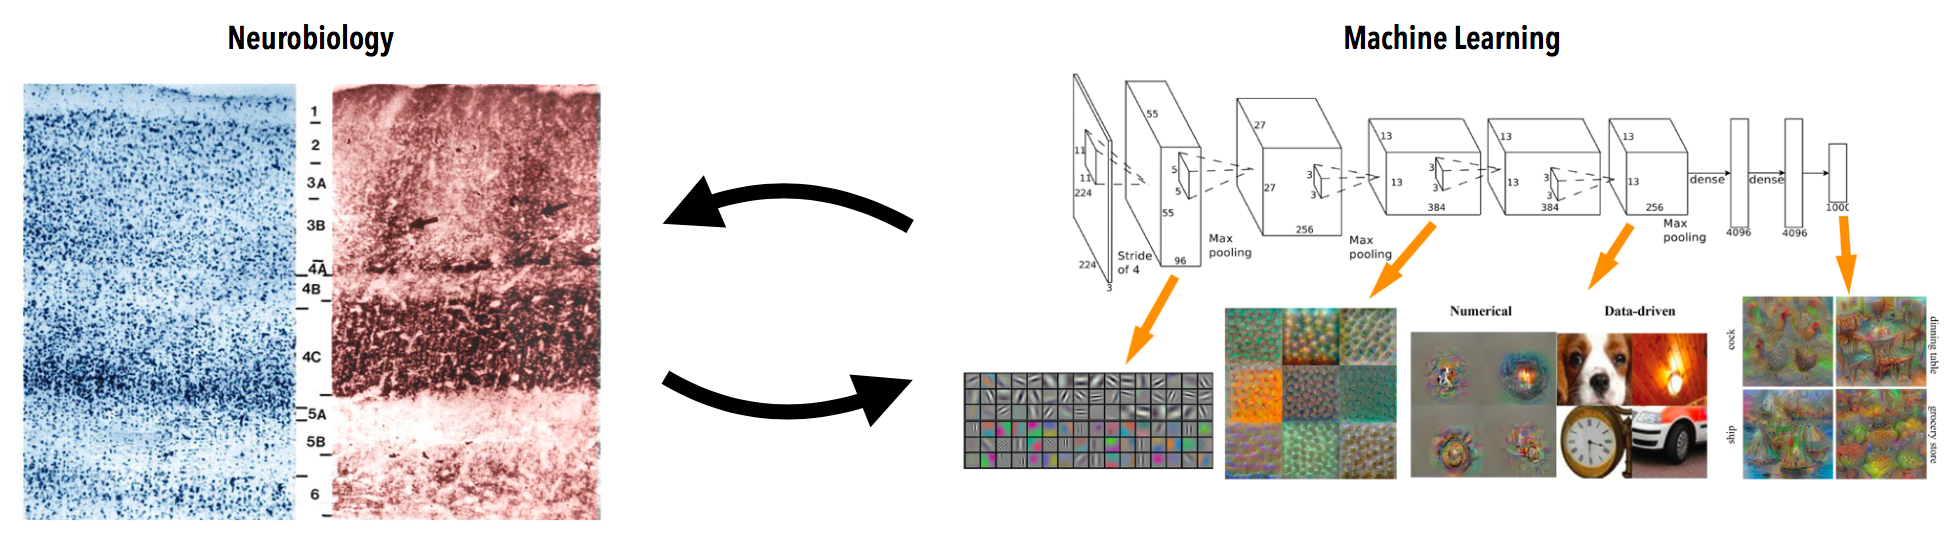
\includegraphics[width=\linewidth]{biology_vs_cnn.png}
  \caption{The Biological Vision (schematic)}
	\label{fig:vision}
\end{figure}

Biological vision is an extremely powerful system which allows humans the ability, and seemingly without effort, to recognize an enormous amount of distinct objects in the world. 
Object detection is extremely difficult and therefore is especially impressive as light intensities can change by levels of magnitude and contrast between foreground and background is so often low. 
In addition, the visual scene changes every time the human body or human eyes move. 
This visual system exhibits a very noisy structure but because it is organized by layers it has inspired the mathematical theory of multilayer neural networks. 
What is remarkable is that even though current machine learning models do not resemble the complexity of its biological pendant, they inherently generalize extremely well. 
Neural networks trained on one specific task can be used to perform detection or segmentation of, seemingly, unrelated objects with relatively minor retraining. 
The reported classification performance is superior to that of humans and the question in regards to their functionality opens an interesting research topic.


GOALS
...reduce the gap between neurobiology and data science to advance the understanding of visual cortex inspired machine learning

CONTRIBUTIONS

- experiments of cleveland mcgill with systematic parametrization and evaluation

- ranking like cleveland mcgill for machine perception?

- many other insights?

- framework





\section{Previous Work}

\textbf{Graphical Perception.} Cleveland and McGill~\cite{cleveland_mcgill} introduce the fundamental concept of \emph{graphical perception} and investigate how different visual attributes and encodings are perceivable by humans. They define \emph{elementary perceptual tasks} as mental-visual stimuli to understand encodings in visualizations. Based on these definitions, the authors propose and perform different experiments such as the \emph{position-angle} experiment which compares bar charts and pie charts, the \emph{position-length} experiment where users judge relations between encoded values in grouped and divided bar charts, and the \emph{bars-and-framed-rectangles} experiment to evaluate Weber's law. Heer and Bostock later reproduced the Cleveland-McGill experiments crowd-sourced on Mechanical Turk~\cite{HeerBostock2010} which lead to follow-up work from Harrison \textit{et al.}~\cite{harrison2013influencing} who replicated the experiments while observing emotional states. Both papers report similar results to Cleveland and McGill which increased our motivation to mimmick their pioneering work. Our experimental setup replicates the original setup of Cleveland and McGill - just instead of humans, we use convolutional neural networks due to the connection with the human visual system. While we focus on Cleveland and McGill's work from 1984, many other excellent articles from the last decades target low-level visual encoding~\cite{bertin1967semiologie,cleveland1985graphical,treisman1988feature, wilkinson2006grammar, carpendale2003considering,widgor_perception2007,munzner2015visualization}.

Interesting are also the rankings of correlation visualization using Weber's law~\cite{harrison2014_webers_law_rank}. This law defines the proportional relation between the initial distribution density and perceivable change. In this paper, we investigate with a simple experiment whether this holds for convolutional neural networks.
\\~\\
%\textbf{Comparing Visual Encodings.} Different visual encodings have advantages or disadvantages and the community does a great job comparing them. Higher-level comparisons include 2D versus 3D vector field and rendering studies~\cite{mckenzie_2d_3d,forsberg2009comparing_3d_vector,laidlaw_2d_vector,borkin2011arteries}, timeseries~\cite{herr2009timeseries} and scatterplots~\cite{tremmel1995visual,Wang_linegraph_vs_scatterplot}. Lower-level experiments target - besides others - open versus closed encodings~\cite{open_vs_closed_shapes}, and several evaluations of color space~\cite{ware1988color,rheingans1992color,Rogowitz2001_colormaps,kindlmann2002color}. While we investigate lower-level visual encodings in this work, we delay colorspace experiments for future work.

\textbf{Computational Visualization Understanding.}

Pineo \textit{et al.}~\cite{Pineo2012_computational_perception} create computational model of human vision based on neural networks and their experiments show that understanding visualization triggers neural activity in high-level areas of cognition. The authors suspect that this level of understanding is produced by low-level neurons performing elementary perceptional tasks. We are further investigating this suspision.
Other work tries to parse infographics by finding higher-level saliency models~\cite{bylinskii2016should}, or by extracting text or key visual elements~\cite{diagram_understanding,kembhavi2016diagram,zoya_text_visual_tags}. However, none of these works focus on computational understanding of lower-level building blocks of visualizations such as curvature, lengths, or position.
\\~\\
\textbf{Visual Cortex Inspired Machine Learning.} 
%Classifiers mimmicking the human visual system are a hot topic and many different architectures, models, and paradigms exist. Feed-forward neural networks 
The human visual cortex is an extremely powerful system which allows the ability, and seemingly without effort, to recognize an enormous amount of distinct objects in the world. This visual system is organized in layers and has inspired the theory of computational classifiers based on multilayer neural networks. Fukushima and Miyake developed the Neocognitron quantitative model~\cite{fukushima1982neocognitron} that ultimately led to the important work of Hinton, Bengio, and LeCun: \textit{deep neural networks}~\cite{lecun2015deep}, visual cortex inspired machine learning.
Nowadays, such classifiers exist with many different architectures. For this paper, we select the traditional \emph{LeNet-5}~\cite{lenet} which was designed to recognize hand-written digits, the VGG19~\cite{simonyan_very_deep2014} classifier with 16 convolutional layers, and the Xception~\cite{xception} classifier with 36 convolutional layers. Selecting these specific networks allows us to compare archtitectures with different depths.
%Object detection is extremely difficult and therefore is especially impressive as light intensities can change by levels of magnitude and contrast between foreground and background is so often low. 
%In addition, the visual scene changes every time the human body or human eyes move. 
%This visual system exhibits a very noisy structure but because it is organized by layers it has inspired the mathematical theory of multilayer neural networks. 

%In 1962 Hubel and Wiesel were the first to begin studying the visual cortex from the standpoint of a neuroscientist. Their experimental findings on cats and macaque monkeys suggested a hierarchy of cells with increasing complexity which was then later transferred to the hierarchical model of different layers. Twenty years later, this insight was translated to the Neocognitron quantitative model, by Fukushima and Miyake, which ultimately led to the important work of Hinton, Bengio, and LeCun in the 1980s. Their work on stochastic gradient descent approximation, and the availability of faster computer hardware then led to today’s deep learning networks. In the last decade, this field has exhibited rapid growth, constant evolution, and new applications in various domains.


%The reported classification performance is superior to that of humans and the question in regards to their functionality opens an interesting research topic.
%Visual cortex inspired machine learning classifiers exist with many different architectures. We select the traditional \emph{LeNet-5}~\cite{lenet} which was designed to recognize hand-written digits, the VGG19~\cite{simonyan_very_deep2014} classifier with 16 convolutional layers, and the Xception~\cite{xception} classifier with 36 convolutional layers. 
%
%What is remarkable is that even though current machine learning models do not resemble the complexity of its biological pendant, they inherently are able to generalize but only after learning thousands of examples. 
%Neural networks trained on one specific task can be used to perform detection or segmentation of, seemingly, unrelated objects with relatively minor retraining~\cite{transfer_learning}. 
%
%
%We think that the biological inspiration of modern convolutional neural networks yields the evaluation of principles of human perception with computers.
%
%
%MLP, LeNet, VGG, ImageNet, XCeption, ResNets etc and work from THomas Serre
%
%
%- https://link.springer.com/chapter/10.1007/978-3-642-14600-8_46
%
%- https://github.com/tidyverse/ggplot2/wiki/Recommended-Reading
%
%- last year's VADL workshop: https://vadl2017.github.io/




\section{Experimental Setup}

We conduct quantitative experiments to measure how different convolutional neural networks perceive low-level visual encodings, such as positions, angles, curvatures, and lengths. We formulate these measurement tasks as logistic regression problems: given a stimuli image of an elementary visualization, the networks must estimate the single quantity present or the ratio between multiple quantities present. 

For each experiment, we use a single factor between-subject design, with the factor being the network used. This lets us evaluate whether different network designs are competitive against existing human perception results. We train each network in a supervised fashion with a mean-squared error (MSE) loss between the ground-truth labels and the network's estimate of the measurement from observing the generated stimuli images. Then, we test each network's ability to generalize to new examples with a separate data, created using the same stimuli generator function but with unseen ground-truth measurements (Section~\ref{sec:data}).

% We define a series of hypotheses prior to each experiment.

\subsection{Networks}
\label{sec:networks}

\noindent{\textbf{Multilayer Perceptron.}} As baseline, we use a multilayer perceptron (MLP), but without the prior convolutional layers as is typical in network designs for solving visual tasks (Fig.~\ref{fig:classifiers}). Our MLP contains a layer of $256$ perceptrons, which are activated as rectified linear units (ReLU)~(Fig.~\ref{fig:classifiers}). We train this layer with dropout (probability $= 0.5$) to prevent overfitting, and then combine these ReLU units to regress our output measurement.
\\~\\
\noindent{\textbf{Convolutional Neural Networks.}} We compare different convolutional neural networks (CNNs) with both `trained from scratch' weights and pre-trained weights on a database of natural images (1000-class ImageNet \cite{imagenet}). These networks are the traditional LeNet-5 with 2 layers, which was designed to recognize hand-written digits~\cite{lenet}; the VGG19 network with 19 layers, which was designed to solve the ImageNet object recognition challenge~\cite{simonyan_very_deep2014}; and the Xception network with 36 layers~\cite{xception}, which was also designed to solve the ImageNet object recognition challenge plus the 15,000-class JFT object recognition challenge~\cite{Hinton2015}. Each of these networks has as its last layers an MLP architecture equivalent to our baseline, and so they act as earlier image and feature processors for this final regressor. Since the networks are of different architectures, the number of trainable parameters changes, with some networks having more capacity than others (Table~\ref{tab:parameters}).

For \emph{VGG19} and \emph{Xception}, we have two variants: the network trained from scratch on elementary perceptual tasks, plus the network using weights that were previously trained on the ImageNet object recognition challenge \emph{except} for the MLP layer. This is intended to produce early-layer features which mimic human vision, and then to see whether they are more or less useful than networks trained from scratch. 
\\~\\
\noindent{\textbf{Optimization.}} All network hyperparameters, optimization methods, and stopping conditions are fixed across networks (Table \ref{tab:parameters}). We train for $1000$ epochs using stochastic gradient descent with Nesterov momentum, but stop early if the loss does not decrease for ten epochs.
\\~\\
\noindent{\textbf{Environment.}} We run all experiments on Tesla X and Tesla V100 graphical processing units. We use the KERAS framework with a TensorFlow backend to train the networks, and use the scikit-image library to generate the stimuli. % and scikit-learn libraries - JT: What do we use this for?

\begin{table}[t]
\centering
\caption{\textbf{Network Training.} We use different feature generators as input to a multilayer perceptron which performs linear regression. This results in different sets of trainable parameters. As a baseline, we also train the MLP directly on the visualization images without any additional feature generation.}
\resizebox{\linewidth}{!}{
\begin{tabular}{lrl}
%	\toprule
%	\makecell{Classifier} & \makecell{Convolutional\\Layers} & \makecell{Trainable\\Parameters} \\
%	\midrule
%	MLP & $0$ & $2,560,513$ \\
%	\emph{LeNet} + MLP & $2$ & $8,026,083$ \\
%	\emph{VGG19} + MLP & $16$ & $21,204,545$ \\
%	\emph{Xception} + MLP & $36$ & $25,580,585$ \\
%	\bottomrule
	\toprule
	Network & \makecell{Trainable\\Parameters} & Optimization \\
	\midrule
	MLP & $2,560,513$ & SGD (Nesterov momentum)\\
	\emph{LeNet} + MLP & $8,026,083$ & Learning rate: $0.0001$\\
	\emph{VGG19} + MLP & $21,204,545$ & Momentum: $0.9$ \\
	\emph{Xception} + MLP & $25,580,585$ & \makecell[tl]{Batchsize: 32\\Epochs: $1000$ (Early Stopping)}\\
	\bottomrule
\end{tabular}
}
\label{tab:parameters}
\vspace{-4mm}
\end{table}
%\begin{figure}[t]
%	\centering
%	  \includegraphics[width=\linewidth]{classifiers.pdf}
%  \caption{The multilayer perceptron (MLP) in our experiments has 256 neurons which are activated as rectified linear units (ReLU). We use Dropout regularization to prevent overfitting. We learn categorical and unordered dependent variables using the softmax function and perform linear regression for continuous variables. The MLP can learn the visualizations directly but we also learn features generated by LeNet (2 conv. layers, filter size $5\time5$), VGG19 trained on ImageNet (16 conv. layers, filter size $3\times3$), or Xception trained on ImageNet (36 conv. layers, filter size $3\times3$) to increase the number of trainable parameters.}
%	\label{fig:classifiers}
%\end{figure}
\begin{figure}[t]
	\centering
	
    \subfloat[Feature Generation]{
		\includegraphics[width=4.8cm,valign=c]{classifier_left.pdf}
		\vphantom{\includegraphics[width=3.5cm,valign=c]{classifier_right.pdf}}
	}
	\hfill
    \subfloat[Multilayer Perceptron]{
		\includegraphics[width=3.5cm,valign=c]{classifier_right.pdf}
	}

  \caption{\textbf{Network Architecture.} The multilayer perceptron (MLP) in our experiments has 256 neurons which are activated as rectified linear units (ReLU). We use Dropout regularization to prevent overfitting. As output, we perform linear regression for continuous variables. The MLP can learn to represent the visualizations directly, but we also learn features generated by LeNet (2 conv. layers, filter size $5\times5$), VGG19 (16 conv. layers, filter size $3\times3$), or Xception (36 conv. layers, filter size $3\times3$) to test different model complexities.}
	\label{fig:classifiers}
\end{figure}

\subsection{Data}
\label{sec:data}

\noindent\textbf{Image Stimuli and Labels} 
We create our stimuli visualizations as 100$\times$100 binary images, rasterized without interpolation. We write a parameterized stimuli generator for each elementary task. The number of possible parameter values differs per experiment, and we summarize these in Table~\ref{tab:encoding_parameters} and Section~\ref{sec:parametrizations}. Before use, we scale the generated images into an unbiased range: images to the range of $-0.5$ to $0.5$. Then, we add subtle random noise (between $0--0.05$) to each pixel to introduce variation which prevents the networks from simply `remembering' each different image.

Each stimuli image also has an associated ground truth label representing the parameter set which generated the image, e.g., the length in pixels of a bar. As before, we scale these labels to the range of $0.0$ to $1.0$, which represent the maximum and minimum values that this parameter can take.
\\~\\
\noindent\textbf{Training/Validation/Test Splits.} For each task, we use 60,000 training images, 20,000 validation images, and 20,000 test images. To create these datasets, we generate stimuli from random parameters and add them to the sets until the target number is reached, while maintaining distinct (random) parameter spaces for each set to ensure that there is no leakage between training and validation/testing.

\subsection{Measures and Analysis}

\noindent\textbf{Cross Validation.} For reproducibility, we perform repeated random sub-sampling validation, also known as Monte Carlo cross-validation, during our experiments. We run every experiment seperately twelve times, and randomly select (without replacement) the $60\%$ of our data as training data, $20\%$ as validation, and $20\%$ as test. 
%Our large data sample size of 100,000 guarantees that every single observation of our parameterizations will be selected at least once (excluding noise patterns). -> JT: No it doesn't.
% Finally, we average the results over the runs. -> JT: Fine, but we'll do distributions anyway, so not worth saying.
\\~\\
\noindent{\textbf{Task Accuracy.}} In their 1984 paper, Cleveland and McGill use the midmean logistic absolute error metric (\emph{MLAE}) to measure perception accuracy. To allow comparison between their human results and our machine results, we also use MLAE as a presentation metric:
\begin{equation}
	\textnormal{MLAE} = log_2( | \textnormal{predicted percent} - \textnormal{true percent} | + .125)
\end{equation}
In addition to this metric, we also calculate standard error metrics such as the mean squared error (\emph{MSE}) and the mean absolute error (\emph{MAE}). This allow a more direct comparison of percent errors. However, please note that our networks were trained using MSE loss and not directly with MLAE.
\\~\\
\noindent{\textbf{Task Confidence Intervals.}} We follow Cleveland and McGill and present $95\%$ confidence intervals. However, as our networks but rather than performing bootstrapping, we approximate the value of the $97.5$ percentile point of the normal distribution for simplicity. JT: What? Why 97.5\% ? Why not 95\% ?
\\~\\
\noindent{\textbf{Confirmatory Data Analysis.}} To accept or reject our hypotheses, we analyze dependent variables using analysis of variance (ANOVA) followed by parametric tests. JT: Which tests?
\\~\\
\noindent{\textbf{Training Efficiency.}} We use the training convergence rate as a measure of how easy or hard a particular task is for the network to learn to solve. This is defined as the MSE loss decrease per training epoch, which is an indicator of the training efficiency of the network with respect to the visual encoding.
\\~\\
\noindent\textbf{Network Generalizability.} We evaluate generalizability by asking a network previously trained upon one task parameterization to answer quetsions about the same type of task stimuli but with more complex parameterization, e.g., estimating bar length without and with changes in stroke width.

Further, some experiments compare different visual encoding types, e.g., bar plot vs.~stacked bar plot. We train and evaluate individual networks for each parameterization, plus we also train and evaluate a networks on stimuli across the different types. This single decision-making software better mimics the judgements that a human would be able to make. 
%This scenario affects the optimization process and result in networks with more flexible knowledge with the caveat of longer training times. -> JT: Save it for the results discussion.


% !TeX root = paper.tex
\section{Experiment: Elementary Perceptual Tasks}

Cleveland and McGill describe a set of elementary graphical perceptual tasks across ten encodings, where each encodes a quantitative variable in a graphical element or visual mark~\cite{cleveland_mcgill,cleveland1985graphical}. These tasks are the low-level building blocks for information visualizations (Table~\ref{tab:encoding_parameters}): estimating position on a common scale, position on non-aligned scales, length, direction (or slope), angle, area, volume, curvature,  shading (or ink density), and color saturation. As human color perception is complex, and because Cleveland and McGill perform no experiments with it, for now we leave it for future work. 

For the remaining nine tasks, we create visualizations as 100$\times$100 raster images, and test whether each of our networks is able to regress values from the images. As discussed in Section~\ref{sec:measuresandanalysis}, we generate multiple parameterizations for each elementary perceptual task to allow us to increase the number of parameters that the networks must estimate, and to measure performance as we move closer towards a general representation of visual marks. For instance, for \emph{Position Common Scale}, first we only vary the $y$-position of the spot to estimate against the scale, then we include translation along the x-axis, and then we vary the size of the spot size. These parameterizations are still simple---each increase is only slightly more complex for a human to solve---but it rapidly increases the number of possible images that the network must `learn' (Table~\ref{tab:encoding_parameters}).

JT: Write something about comparison to Cleveland and McGill's 1985 experimental encoding?

JT: Write something more intelligent about the different kinds of parameter variations.

%Cleveland and McGill did not explicitly test human perception of single instances of these encodings. -> JT: We now know this isn't true.

%\begin{figure}[t]
%	  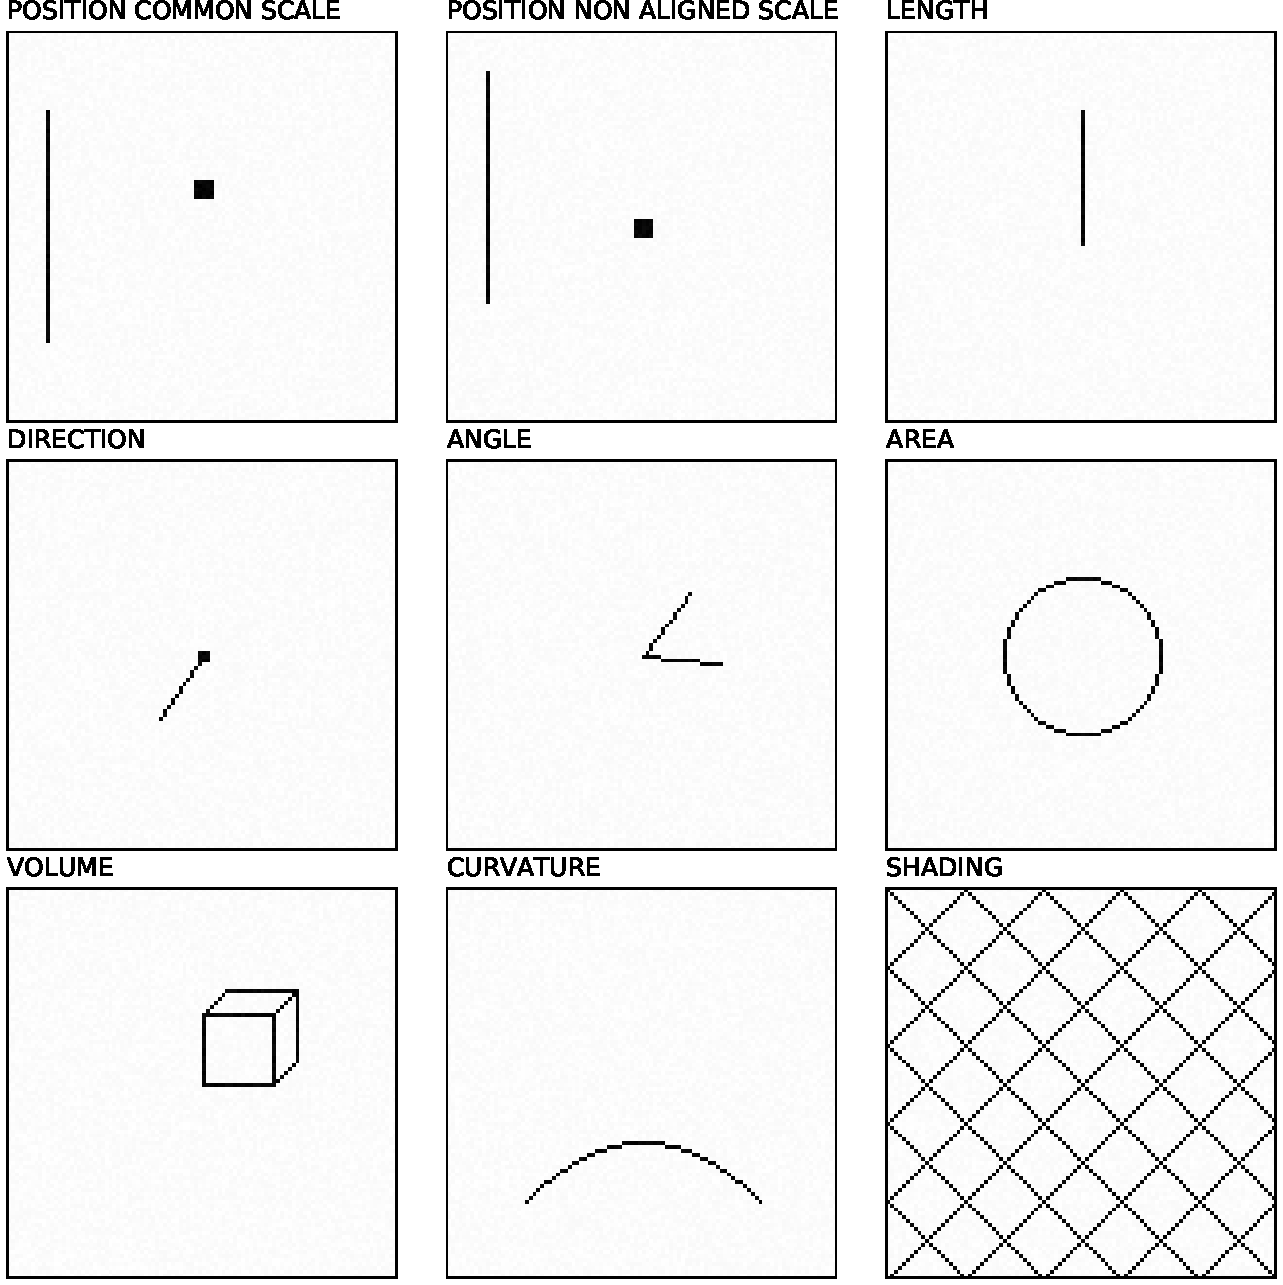
\includegraphics[width=\linewidth]{figure1_overview.pdf}
%  \caption{\textbf{Elementary Perceptual Tasks.} Rasterized visualizations of the elementary perceptual tasks as defined by Cleveland and McGill~\cite{cleveland_mcgill} (color saturation excluded). We vary the parameters of each perceptual task and then assess the interpretability of feed-forward neural networks.}
%	\label{fig:elementary_perceptual_tasks}
%\end{figure}



\begin{table}[!ht]
\centering
\caption{\textbf{Elementary Perceptual Tasks.} Rasterized visualizations of the elementary perceptual tasks as defined by Cleveland and McGill~\cite{cleveland_mcgill} (color saturation excluded). We sequentially increase the number of parameters for every task (e.g., by adding translation). This introduces variability and creates increasingly more complex datasets.}
\resizebox{\linewidth}{!}{
\begin{tabular}{lllr}
	\toprule
	\multicolumn{2}{l}{Elementary Perceptual Task} & ~ & Permutations\\
	\midrule
	\raisebox{-.85\height}{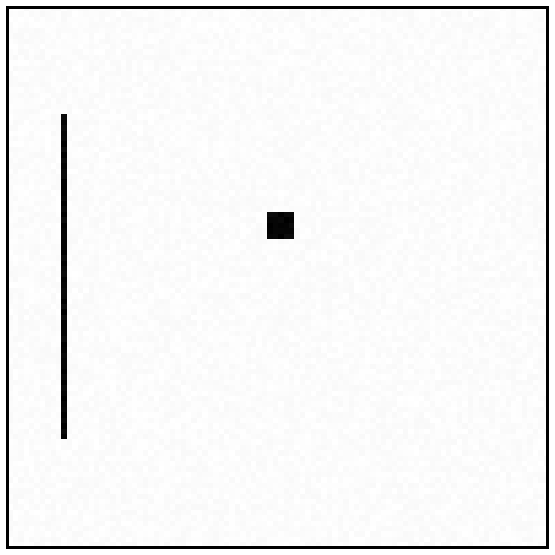
\includegraphics[width=.5in]{position_common_scale.pdf}} & \makecell[tl]{\emph{Position Common Scale}\\~~~Position Y\\~~~+ Position X \\~~~+ Spot Size \\} &~& \makecell[tr]{~\\ $60$ \\ $3,600$ \\ $216,00$}\\

	\midrule
	\raisebox{-.85\height}{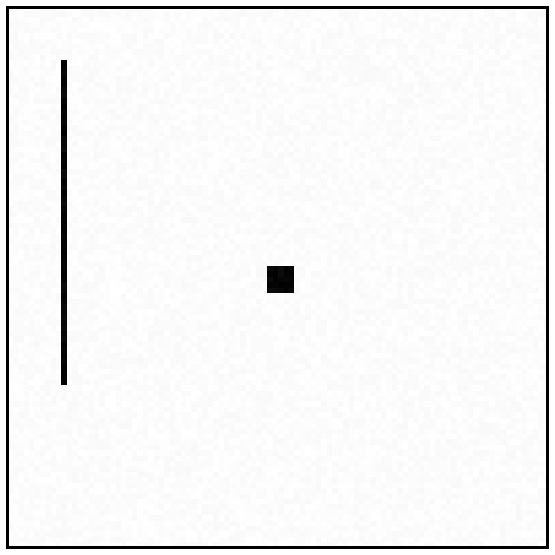
\includegraphics[width=.5in]{position_non_aligned_scale.pdf}} & \makecell[tl]{\emph{Position Non-Aligned Scale}\\~~~Position Y\\~~~+ Position X \\~~~+ Spot Size \\} &~& \makecell[tr]{~\\ $600$ \\ $36,000$ \\ $216,000$}\\

	\midrule
	\raisebox{-.95\height}{
\includegraphics[width=.5in]{length.pdf}} & \makecell[tl]{\emph{Length}\\~~~Length\\~~~+ Position Y \\~~~+ Position X \\~~~+ Width} &~& \makecell[tr]{ ~\\$60$ \\ $2,400$ \\ $144,000$\\$864,000$}\\

	\midrule
	\raisebox{-.85\height}{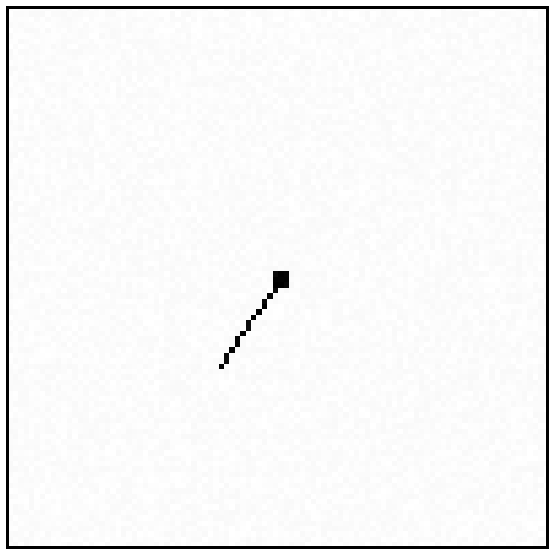
\includegraphics[width=.5in]{direction.pdf}} & \makecell[tl]{\emph{Direction}\\~~~Angle\\~~~+ Position Y \\~~~+ Position X} &~& \makecell[tr]{ ~\\$360$ \\ $21,600$ \\ $1,296,000$}\\

	\midrule
	\raisebox{-.85\height}{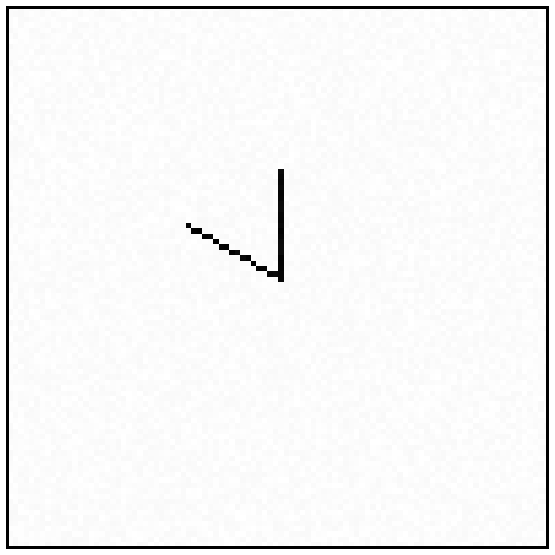
\includegraphics[width=.5in]{angle.pdf}} & \makecell[tl]{\emph{Angle}\\~~~Angle\\~~~+ Position Y \\~~~+ Position X} &~& \makecell[tr]{ ~\\$90$ \\ $5,400$ \\ $324,000$}\\

	\midrule
	\raisebox{-.85\height}{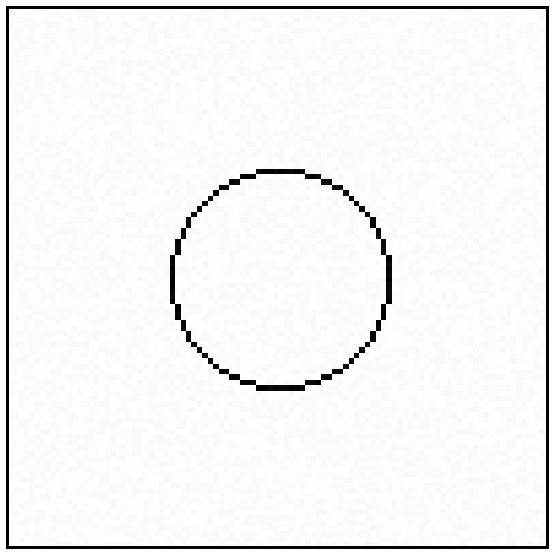
\includegraphics[width=.5in]{area.pdf}} & \makecell[tl]{\emph{Area}\\~~~Radius\\~~~+ Position Y \\~~~+ Position X} &~& \makecell[tr]{ ~\\$40$ \\ $800$ \\ $16,000$}\\

	\midrule
	\raisebox{-.85\height}{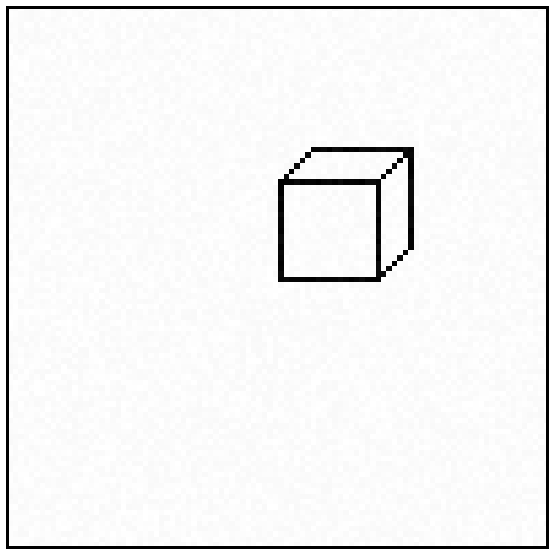
\includegraphics[width=.5in]{volume.pdf}} & \makecell[tl]{\emph{Volume}\\~~~Cube Sidelength\\~~~+ Position Y \\~~~+ Position X} &~& \makecell[tr]{ ~\\$20$ \\ $400$ \\ $8,000$}\\
	
	\midrule
	\raisebox{-.85\height}{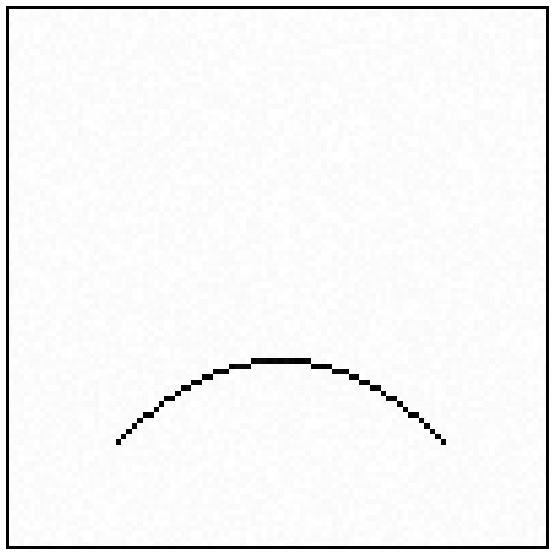
\includegraphics[width=.5in]{curvature.pdf}} & \makecell[tl]{\emph{Curvature}\\~~~Midpoint Curvature\\~~~+ Position Y \\~~~+ Position X} &~& \makecell[tr]{ ~\\$80$ \\ $1,600$ \\ $64,000$}\\	

	\midrule
	\raisebox{-.85\height}{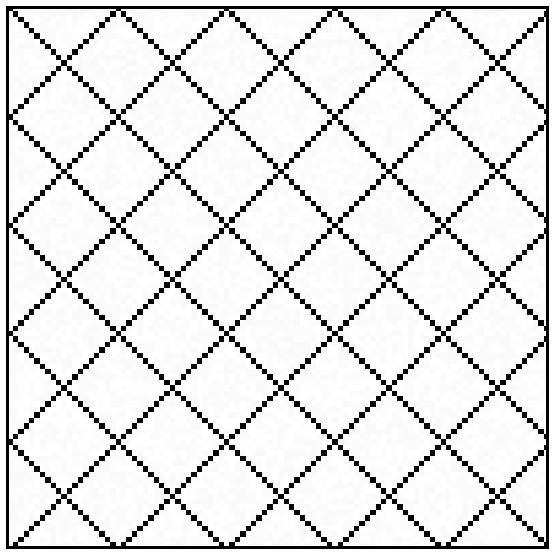
\includegraphics[width=.5in]{shading.pdf}} & \makecell[tl]{\emph{Shading}\\~~~Density\\~~~+ Position Y \\~~~+ Position X} &~& \makecell[tr]{ ~\\$100$ \\ $2,000$ \\ $40,000$}\\	
%	
	\bottomrule
\end{tabular}
}
\label{tab:encoding_parameters}
\end{table}



%
\subsection{Hypotheses}

We state four hypotheses for the elementary perceptual task experiment:

\begin{itemize}
	\item \textbf{H1.1} \textbf{The CNNs tested will be able to regress quantitative variables from graphical elements.} We parametrize different visual encodings (Table~\ref{tab:encoding_parameters}) and test whether the CNNs can measure them, and relate the results to accuracies obtained by humans on similar tasks.
	\item \textbf{H1.2} \textbf{Computed perceptual performance is dependent on network architexture.} We evaluate multiple regressors with different numbers of trainable parameters. We expect a more complex network (with a higher number of trainable parameters) to perform better on elementary perceptual tasks.
	\item \textbf{H1.3} \textbf{Some visual encodings will be easier to learn than others for the CNNs tested.} Cleveland and McGill order the elementary perceptual tasks by accuracy. We investigate whether this order is also relevant for computing graphical perception.
	\item \textbf{H1.4} \textbf{Networks trained on perceptual tasks can generalize to more and less complex variations of the same task.} Empirical evidence suggests that CNNs are able to generalize by interpolating between different training data points. This property allows them to perform on variations of a similar perceptual task. We create visual representations of the elementary perceptual tasks with different variability, and expect that networks will be able to generalize when presented with slight task variations.
\end{itemize}

%	
%	We suspect that CNNs are able to 'learn` absolute quantities encoded using low-level visual 
%	
%	While much simpler models than their biological pendant, convolutional neural networks are heavily influenced by our biological knowledge of the visual system. Such classifiers therefor follow the same principles as human perception.


\subsection{Results}

%While the performance varies for the different encodings, we observe for all networks performance similar to the measured human performance by Cleveland and McGill~\cite{cleveland1985graphical}. These results confirm our initial hypotheses.
\noindent{\textbf{Overall Accuracy.}} The tested CNNs and MLP are able to regress the visually encoded quantities in most cases (Fig.~\ref{fig:figure1_results}), with average error across all classifiers and tasks as \textit{MLAE}$=1.597$ ($SD=0.394$). % and \textit{MAE}=$2.89$ ($SD=0.848$). 
These values are similar or better than the range of MLAE=$3.02$--$3.82$ ($8-14\%$ error) for a similar experiment by Cleveland and McGill testing human estimation of relations between elementary perceptual tasks~\cite{cleveland1985graphical}. From these results, we \textbf{accept H1.1}.
\\~\\
\noindent{\textbf{Comparing Networks.}} 
Across network architectures and training schemes, there is considerable difference in performance. In order of decreasing error: 
The MLP has \textit{MLAE}$=2.943$ ($SD=0.857$), 
for LeNet $2.125$ ($SD=0.38$), 
Xception trained on ImageNet $1.627$ ($SD=0.462$), 
Xception trained from scratch $1.504$ ($SD=0.493$),
VGG19 trained on ImageNet $0.979$ ($SD=0.581$), 
and VGG19 trained from scratch $0.404$ ($SD=0.407$).

Across tasks, we compare the average regression performances for our networks and report the effect of the network as statistically significant ($F_{5,48}=20.392,p<0.01$). Post hoc comparisons show that the differences between LeNet and the VGG19 network, independent of the used weights, are significant ($t_48=4.674,p<0.01$). VGG19 from scratch and Xception (both versions) perform significantly differently, with Xception from scratch ($t_48=4.87,p<0.01$) and Xception with ImageNet weights ($t_48=5.621,p<0.01$). However, differences between LeNet and both Xception networks are not significant. Taken collectively, we \textbf{partially accept H1.2}, in that more tunable parameters does not automatically infer greater performance.
\\~\\
\noindent{\textbf{Ranking of Visual Encodings.}} Cleveland and McGill provide an ordering of elementary visual encodings based on theoretical arguments and experimental results. We compare their ranking with rankings of our networks in Table~\ref{tab:ranking}. We note that the rankings between networks using ImageNet weights is identical; however, overall, there is significant variability, and we \textbf{reject H1.3}. 

%Observing Figure~\ref{fig:figure1_results}, -> JT: we should do this.

%Since such a ranking see,s to heavily depend on the used regressor, the weights, and the initialization, we do not think a generalized ranking can be created and \textbf{reject H1.3}.

\begin{table}[tb]
\centering
\caption{\textbf{Ranking of Elementary Perceptual Tasks.} We create a ranking of the elementary perceptual tasks for all of our networks. We report midmean logistic absolute errors (MLAE) for each network averaged across multiple runs on the most complex parametrization of the individual stimuli. The VGG19 network performs best compared on all tasks. For human performance, we report the ranking of Cleveland and McGill~\cite{cleveland_mcgill}. The VGG19 * and Xception * networks use ImageNet weights and yield identical rankings.}
\resizebox{\linewidth}{!}{
\begin{tabular}{cllllll}
\toprule
Human (CMcG) & MLP & LeNet & VGG19 * & \textbf{VGG19} & Xception * & Xception \\
\midrule
\multicolumn{7}{l}{\emph{Position Common Scale}} \\
1. & 7. (3.84) & 2. (1.36) & 5. (1.02) & \textbf{3.} (-0.04) & 5. (1.65) & 1. (1.04)\\
\multicolumn{7}{l}{\emph{Position Non aligned Scale}} \\
2. & 6. (3.61) & 1. (1.35) & 6. (1.09) & \textbf{5.} (0.26) & 6. (1.71) & 2. (1.06)\\
\multicolumn{7}{l}{\emph{Length}} \\
3. & 1. (1.99) & 8. (3.19) & 4. (0.87) & \textbf{2.} (-0.14) & 4. (1.59) & 3. (1.11) \\
\multicolumn{7}{l}{\emph{Direction}} \\
3. & 9. (4.65) & 7. (3.07) & 9. (2.84) & \textbf{8.} (0.92) & 9. (3.46) & 6. (1.57) \\
\multicolumn{7}{l}{\emph{Angle}} \\
3. & 8. (4.61) & 9. (3.33) & 8. (2.31) & \textbf{9.} (0.99) & 8. (2.60) & 7. (1.72) \\
\multicolumn{7}{l}{\emph{Area}} \\
4. & 2. (2.01) & 5. (2.21) & 1. (0.49) & \textbf{1.} (-0.17) & 1. (0.80) & 5. (1.38) \\
\multicolumn{7}{l}{\emph{Volume}} \\
5. & 4. (2.38) & 4. (1.91) & 7. (1.16) & \textbf{7.} (0.87) & 7. (2.03) & 9. (2.10) \\
\multicolumn{7}{l}{\emph{Curvature}} \\
5. & 3. (2.34) & 3. (1.81) & 2. (0.71) & \textbf{6.} (0.28) & 2. (1.17) & 4. (1.13) \\
\multicolumn{7}{l}{\emph{Shading}} \\
6. & 5. (3.04) & 6. (2.23) & 3. (0.73) & \textbf{4.} (0.14) & 3. (1.57) & 8. (1.82) \\

% 
%\makecell[tl]{\emph{Position}\\~~\emph{Non-aligned Scale}} & 1 & 1 & 2 & 3 & \textbf{4} & 5 & 6 \\
%\makecell[tl]{\emph{Length}} & 1 & 1 & 2 & 3 & \textbf{4} & 5 & 6 \\
%\makecell[tl]{\emph{Direction}} & 1 & 1 & 2 & 3 & \textbf{4} & 5 & 6 \\
%\makecell[tl]{\emph{Angle}} & 1 & 1 & 2 & 3 & \textbf{4} & 5 & 6 \\
%\makecell[tl]{\emph{Area}} & 1 & 1 & 2 & 3 & \textbf{4} & 5 & 6 \\
%\makecell[tl]{\emph{Volume}} & 1 & 1 & 2 & 3 & \textbf{4} & 5 & 6 \\
%\makecell[tl]{\emph{Curvature}} & 1 & 1 & 2 & 3 & \textbf{4} & 5 & 6 \\
%\makecell[tl]{\emph{Shading}} & 1 & 1 & 2 & 3 & \textbf{4} & 5 & 6 \\
%\begin{tabular}{ll}
%	\toprule
%	Task & \begin{tabular}{ccccccc}
%			Human & MLP & LeNet & VGG19 * & VGG19 & Xception * & Xception
%			\end{tabular}\\
%	\midrule
%	\raisebox{-.85\height}{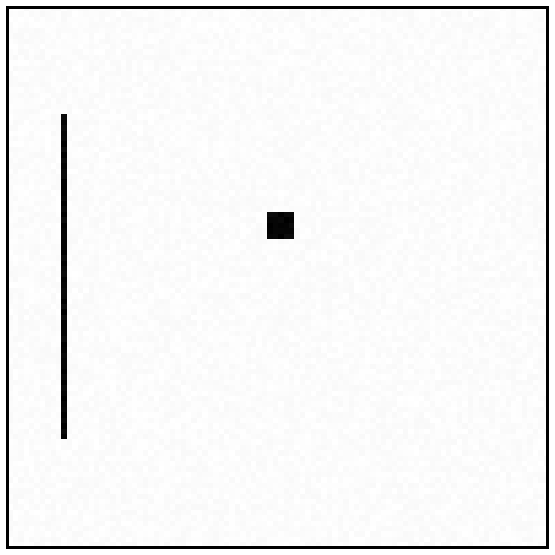
\includegraphics[width=.5in]{position_common_scale.pdf}} & \makecell[tl]{\emph{Position Common Scale}\\ \begin{tabular}{ccccccc}
%
%\end{tabular}} \\
%
%	\midrule
%	\raisebox{-.85\height}{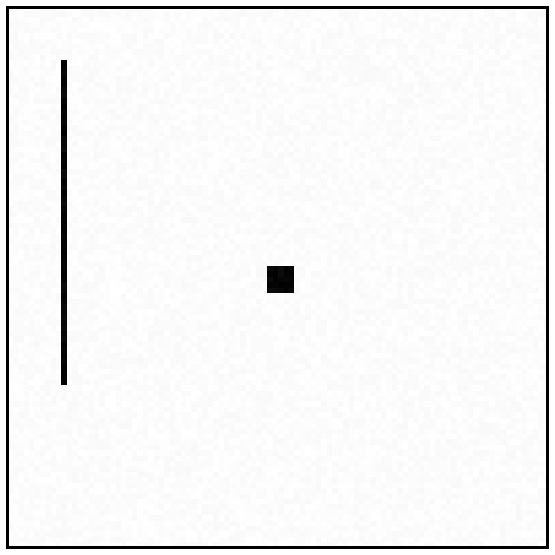
\includegraphics[width=.5in]{position_non_aligned_scale.pdf}} & \makecell[tl]{\emph{Position Non-Aligned Scale}\\~~~Position Y\\~~~+ Position X \\~~~+ Spot Size \\} &~& \makecell[tr]{~\\ $600$ \\ $36,000$ \\ $216,000$}\\
%
%	\midrule
%	\raisebox{-.95\height}{
\includegraphics[width=.5in]{length.pdf}} & \makecell[tl]{\emph{Length}\\~~~Length\\~~~+ Position Y \\~~~+ Position X \\~~~+ Width} &~& \makecell[tr]{ ~\\$60$ \\ $2,400$ \\ $144,000$\\$864,000$}\\
%
%	\midrule
%	\raisebox{-.85\height}{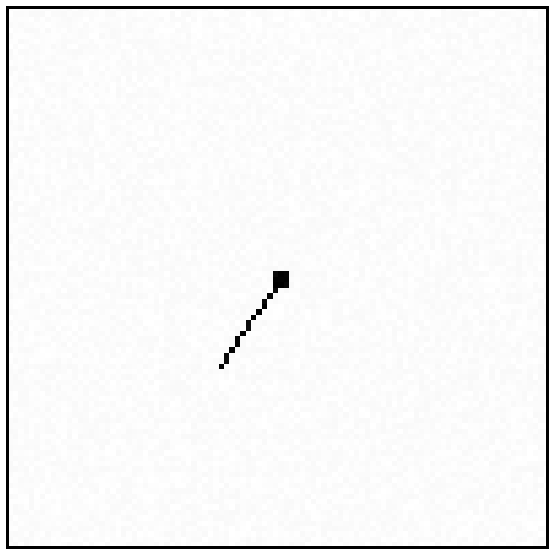
\includegraphics[width=.5in]{direction.pdf}} & \makecell[tl]{\emph{Direction}\\~~~Angle\\~~~+ Position Y \\~~~+ Position X} &~& \makecell[tr]{ ~\\$360$ \\ $21,600$ \\ $1,296,000$}\\
%
%	\midrule
%	\raisebox{-.85\height}{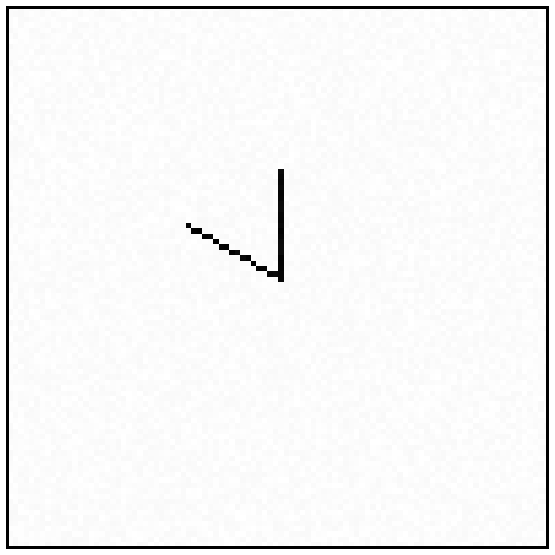
\includegraphics[width=.5in]{angle.pdf}} & \makecell[tl]{\emph{Angle}\\~~~Angle\\~~~+ Position Y \\~~~+ Position X} &~& \makecell[tr]{ ~\\$90$ \\ $5,400$ \\ $324,000$}\\
%
%	\midrule
%	\raisebox{-.85\height}{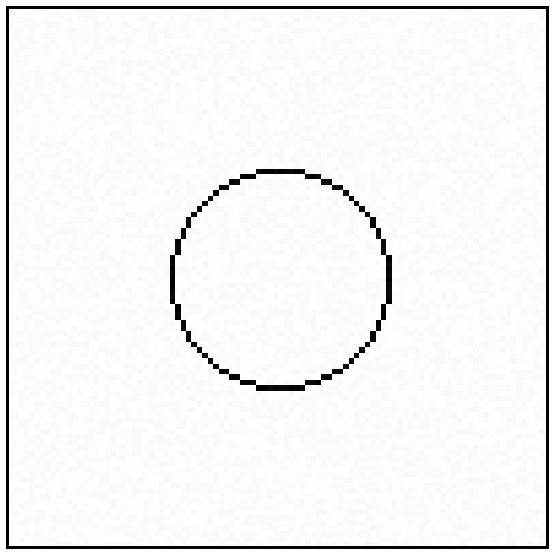
\includegraphics[width=.5in]{area.pdf}} & \makecell[tl]{\emph{Area}\\~~~Radius\\~~~+ Position Y \\~~~+ Position X} &~& \makecell[tr]{ ~\\$40$ \\ $800$ \\ $16,000$}\\
%
%	\midrule
%	\raisebox{-.85\height}{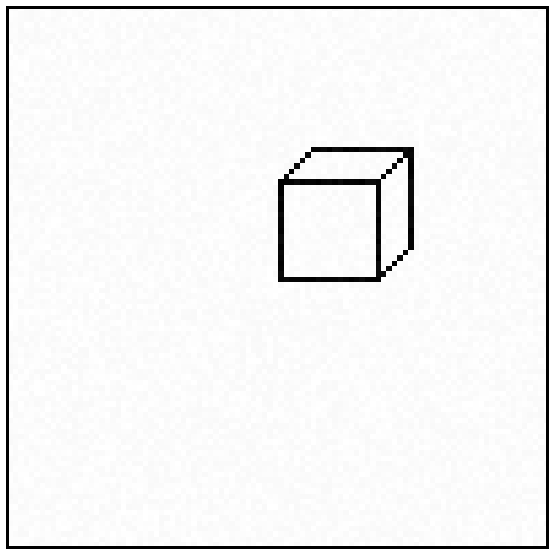
\includegraphics[width=.5in]{volume.pdf}} & \makecell[tl]{\emph{Volume}\\~~~Cube Sidelength\\~~~+ Position Y \\~~~+ Position X} &~& \makecell[tr]{ ~\\$20$ \\ $400$ \\ $8,000$}\\
%	
%	\midrule
%	\raisebox{-.85\height}{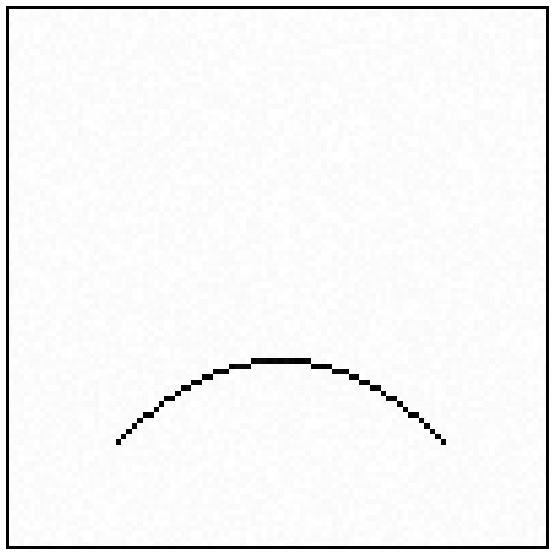
\includegraphics[width=.5in]{curvature.pdf}} & \makecell[tl]{\emph{Curvature}\\~~~Midpoint Curvature\\~~~+ Position Y \\~~~+ Position X} &~& \makecell[tr]{ ~\\$80$ \\ $1,600$ \\ $64,000$}\\	
%
%	\midrule
%	\raisebox{-.85\height}{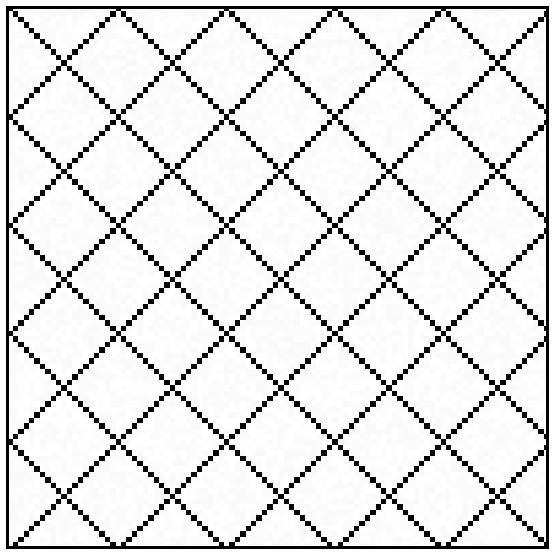
\includegraphics[width=.5in]{shading.pdf}} & \makecell[tl]{\emph{Shading}\\~~~Density\\~~~+ Position Y \\~~~+ Position X} &~& \makecell[tr]{ ~\\$100$ \\ $2,000$ \\ $40,000$}\\	

	\bottomrule
\end{tabular}
}
\label{tab:ranking}
\end{table}

\begin{figure}[!ht]
	\centering
	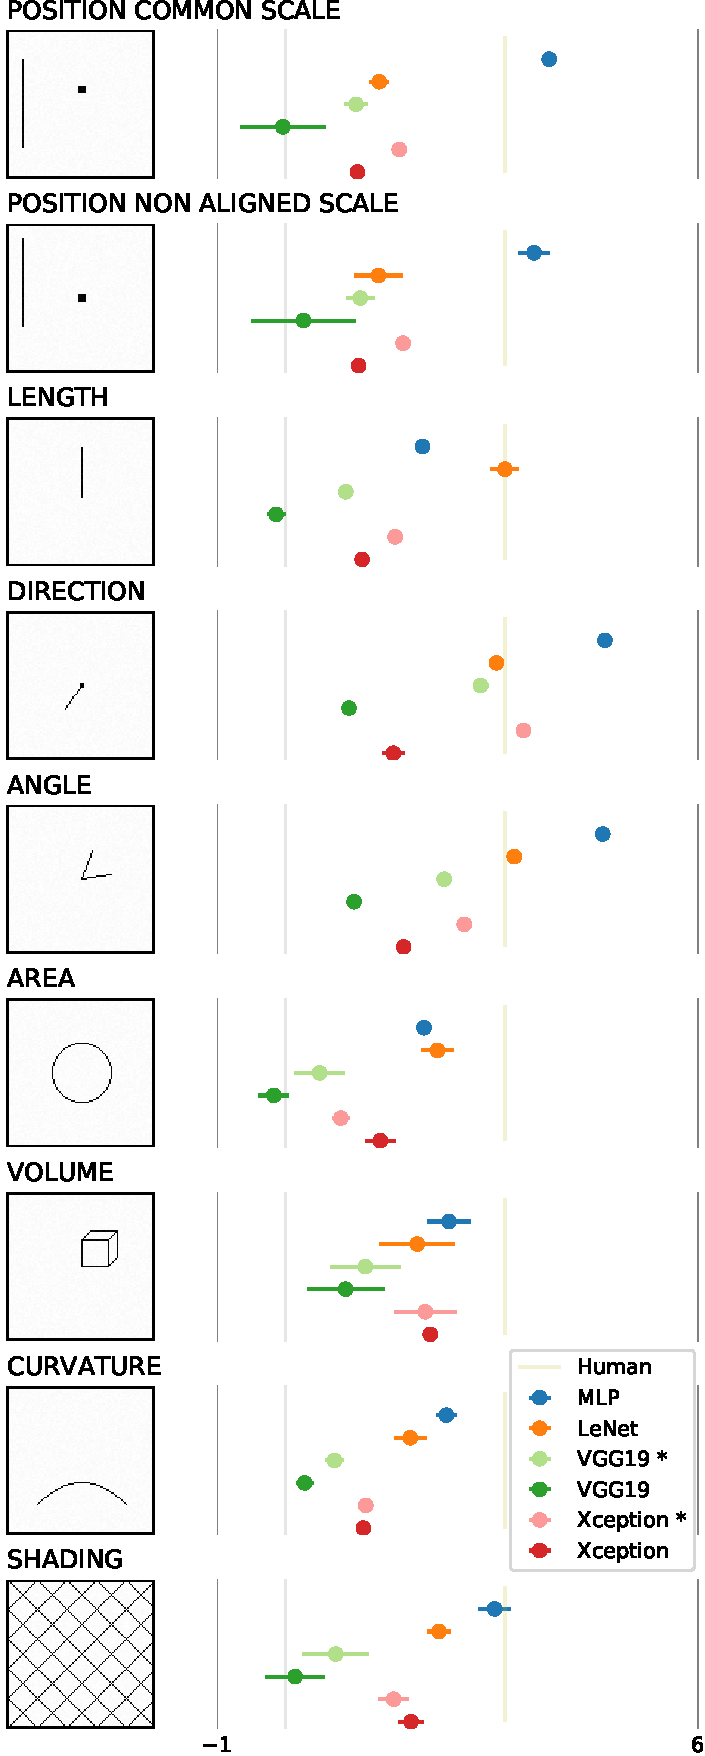
\includegraphics[width=.8\linewidth]{figure1_slim_only_last.pdf}
%	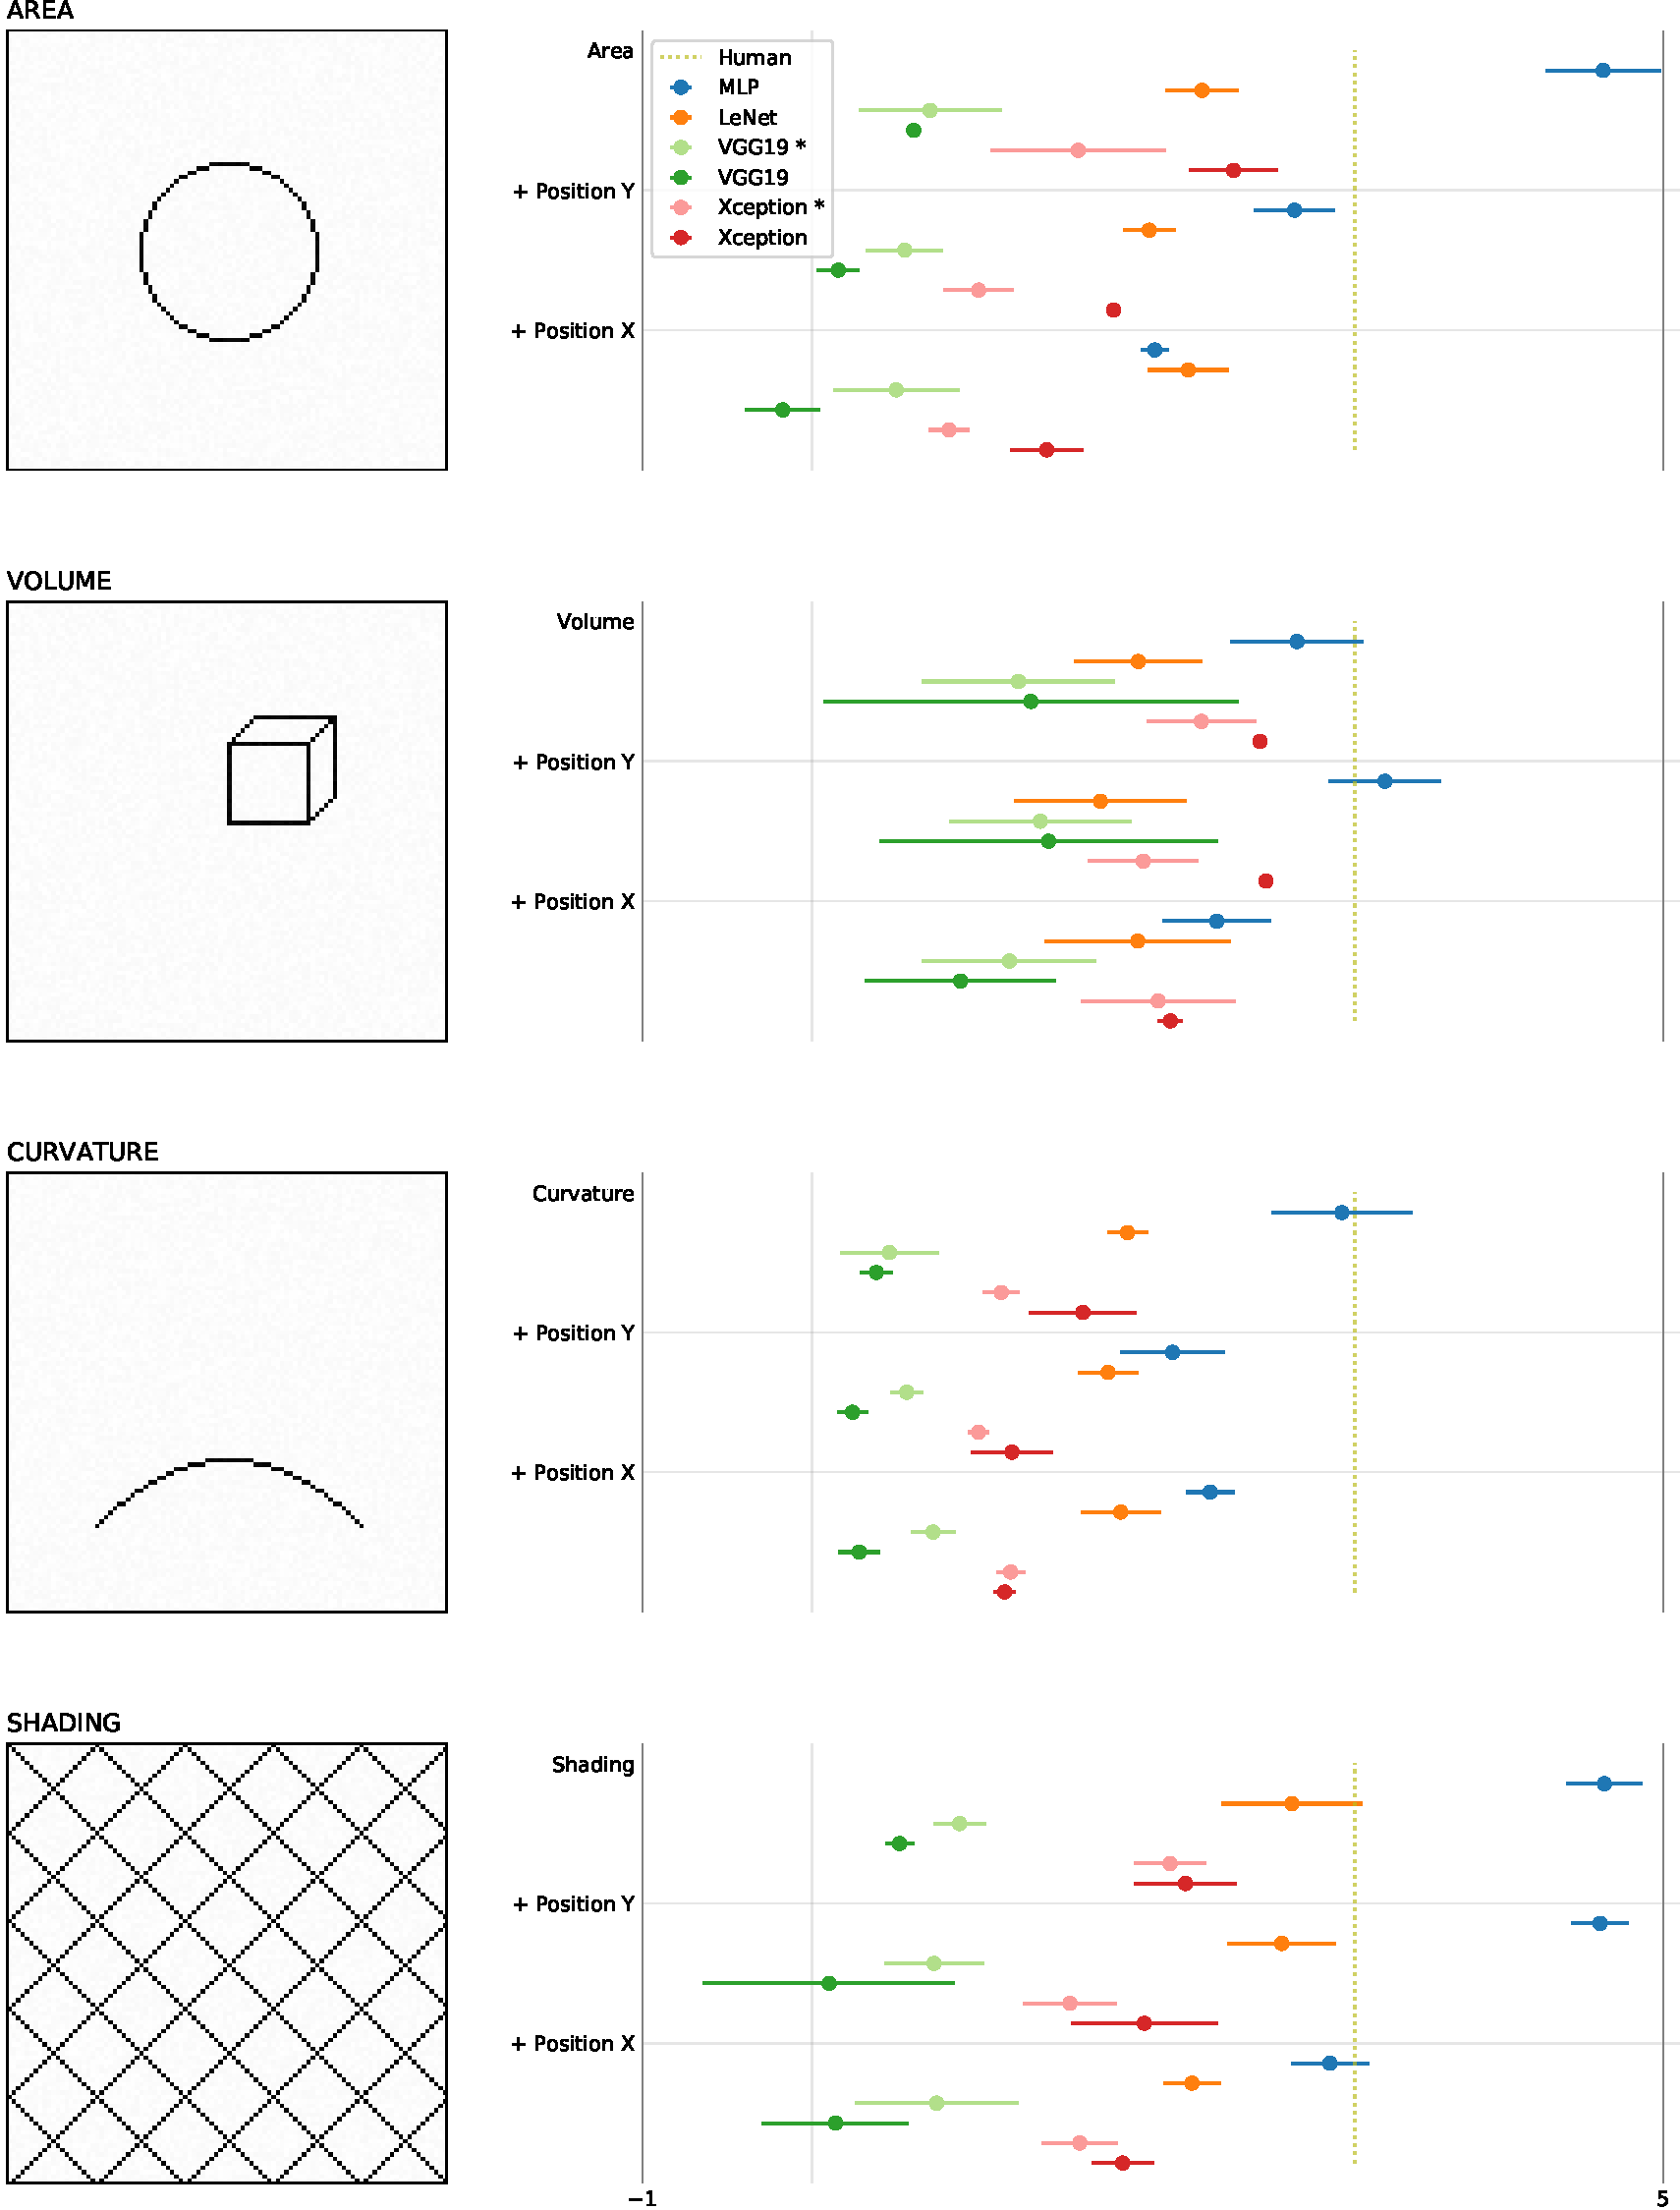
\includegraphics[width=0.48\linewidth]{figure1_slim_right.pdf}
	\caption{\textbf{Elementary perceptual tasks results for most complex task parameterization.} \emph{Left:} Example stimuli image. \emph{Right:} MLAE and 95\% confidence intervals for different networks. The * indicates networks which use ImageNet weights up until the MLP, rather than being trained from scratch.}
	\label{fig:figure1_results}
\end{figure}

\noindent{\textbf{Cross-classifier Variability and Network Generalizability.}} We measure regression performance across classifiers trained on the different parameterizations of the elementary perceptual tasks. Looking at the results in Fig.~\ref{fig:cross_network}, we can observe that even slight variations of an encoding such as added translation in Y or X drastically increases the error. We think that the networks are not really learning concepts of perception but rather learn the variation of pixel values.

\begin{figure}[!ht]
	\centering
	  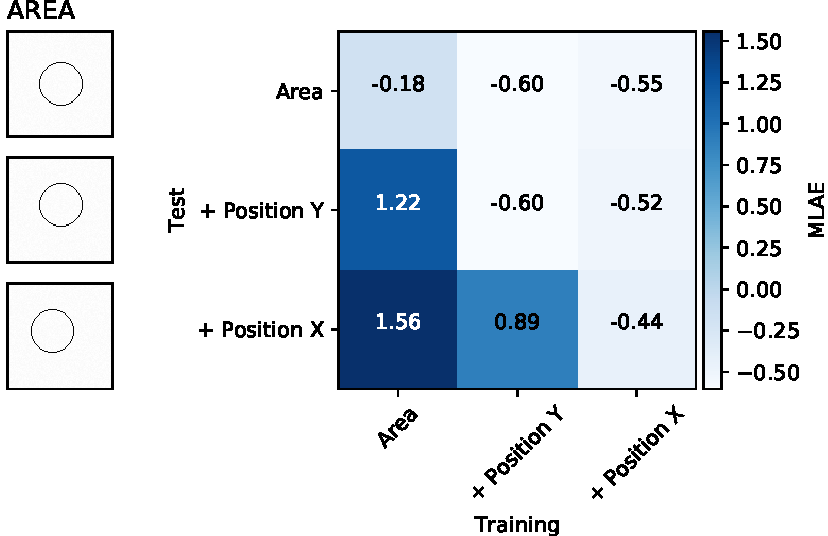
\includegraphics[width=.75\linewidth]{cross_network_small_VGG19_area.pdf}
	  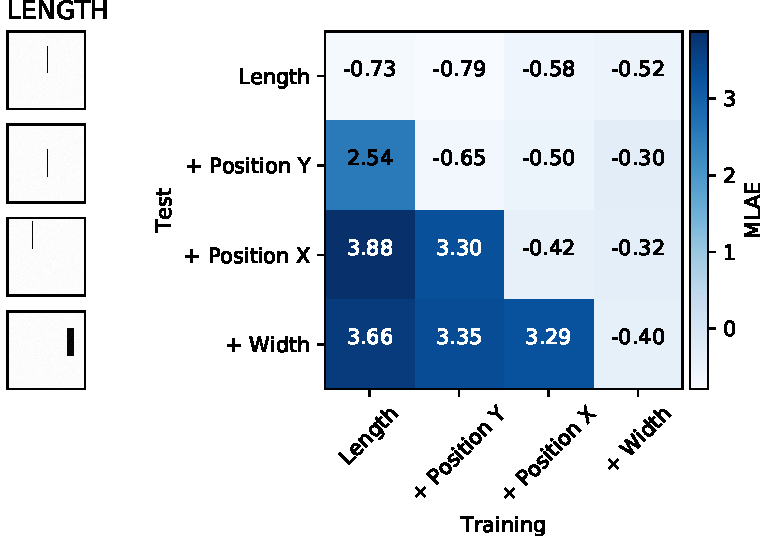
\includegraphics[width=.75\linewidth]{cross_network_small_VGG19_length.pdf}
	  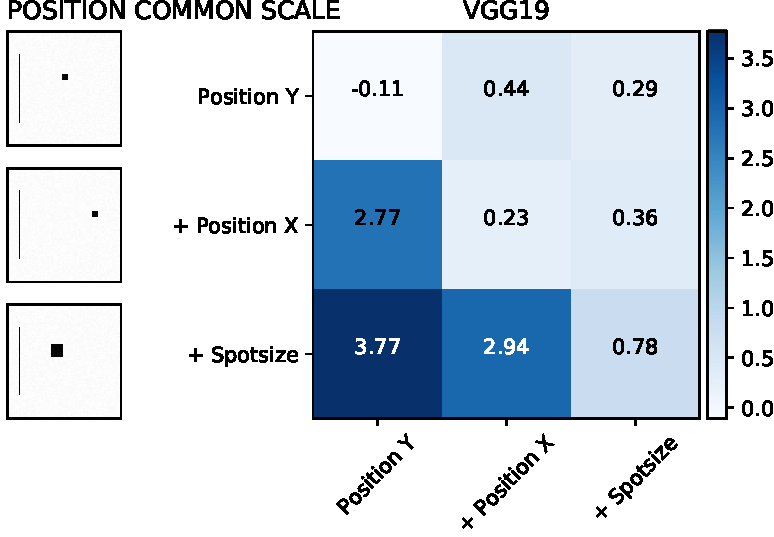
\includegraphics[width=.75\linewidth]{cross_network_small_VGG19_position_common_scale.pdf}
	  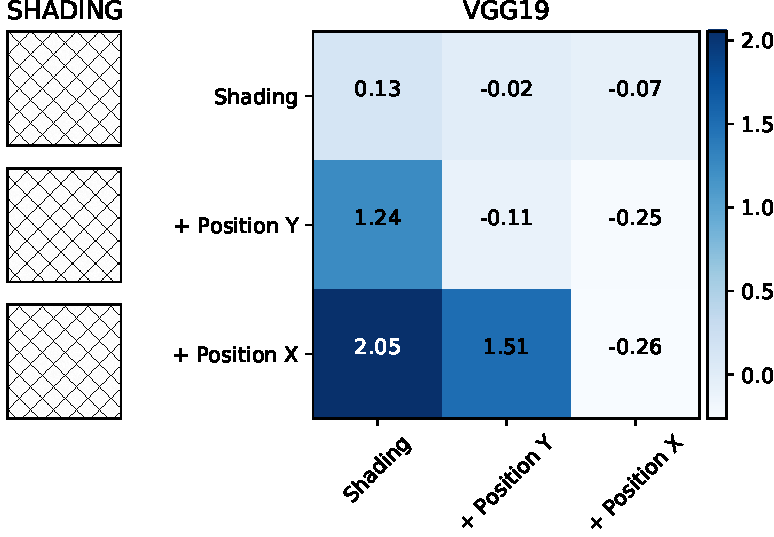
\includegraphics[width=.75\linewidth]{cross_network_small_VGG19_shading.pdf}
  \caption{\textbf{Cross-classifier variability for perceptual tasks.} We use predictions of the VGG19 network trained on different parametrizations of \emph{area}, \emph{length}, \emph{position common scale}, and \emph{shading}. These are the top 4 encodings in the ranking for this network. We measure the mean logistic absolute error (MLAE) -- the lower score, the better. Regressors trained on stimuli with variable position can generalize even if the axis of translation varies. However, if they are trained on fixed positions of the stimuli they are not able to measure translated encodings.}
	\label{fig:cross_network}
\end{figure}



\clearpage
\section{Experiment: Position-Angle}

Cleveland and McGill measure human perception to the ratios of positions and angles through comparisons on bar charts and pie charts~\cite{cleveland_mcgill}. We create rasterized images following Cleveland and McGill's proposed encoding and investigate computational perception of our networks (Figure~\ref{fig:teaser}). These have five bar or pie sectors representing numbers which add to 100, where each is greater than three and smaller than 39. One required change is in the minimal differences between the values: Cleveland and McGill create stimuli where the differences between each number are greater than $0.1$. However, as our networks only take $100\times100$ pixel images as input, we can only minimally represent a difference of $1$ pixel.

Cleveland and McGill ask participants to estimate the ratio of the four smaller bars or sectors to the known and marked largest bar or sector. As such, we mark the largest quantity of the five in each visualization with a single pixel dot, then ask our networks to perform multiple regression and produce the four ratio estimates. Since the position of the largest element changes, we generate the targets such that the largest element is marked with 1 and the smaller elements follow counter-clockwise for the pie chart and to the right for the bar chart. Each of the bar and pie chart visualizations has $878,520$ possible permutations.

% To be successful, the networks essentially first have to find the marked quantity, have the `rolling' encoding figured out, and then estimate the quantities properly.  -> JT: I don't want to prescribe how the network must solve the task. There are other ways to solve it, and this might not be how the network solves the problem.

%\begin{figure}[t]
%	  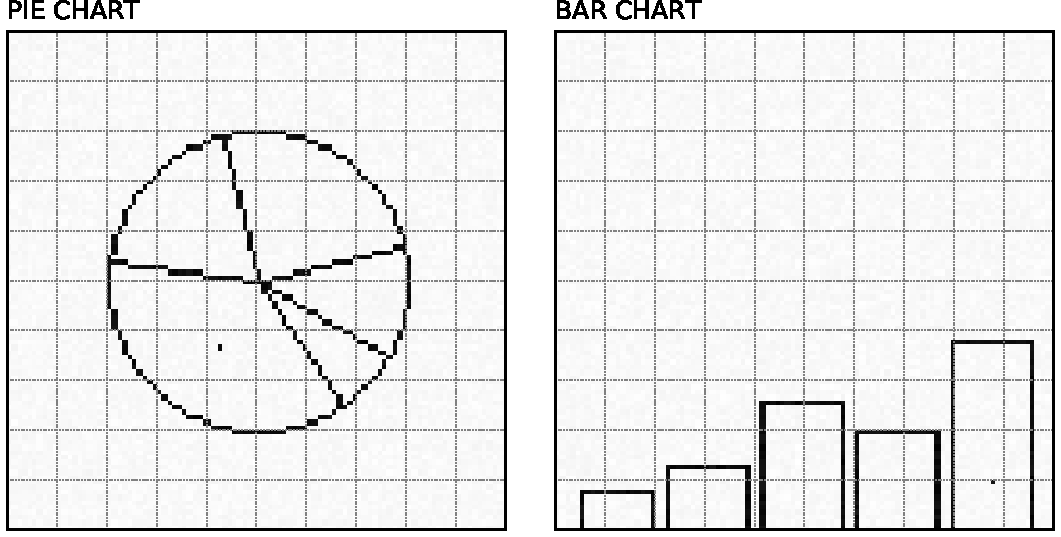
\includegraphics[width=\linewidth]{figure3_overview}
%  \caption{\textbf{Position-Angle Experiment.} We create rasterized visualizations of pie charts and bar charts to follow Cleveland and McGill's position-angle experiment. The experimental task involves the judgement of different encoded values in comparison to the largest encoded values. The pie chart (left) and the bar chart (right) visualize the same data point. In their paper, Cleveland and McGill report less errors using bar charts.}
%	\label{fig:position_angle_experiment}
%\end{figure}
%\begin{table}[h]
%\centering
%\caption{\textbf{Position-Angle Experiment.} We create rasterized visualizations of pie charts and bar charts to follow Cleveland and McGill's position-angle experiment. The experimental task involves the judgement of different encoded values in comparison to the largest encoded values. The pie chart and the bar chart visualize the same data point. In their paper, Cleveland and McGill report less errors using bar charts.}
%\resizebox{\linewidth}{!}{
%\begin{tabular}{lllr}
%	\toprule
%	\multicolumn{2}{l}{~} & ~ & Permutations\\
%
%	\midrule
%	\raisebox{-.85\height}{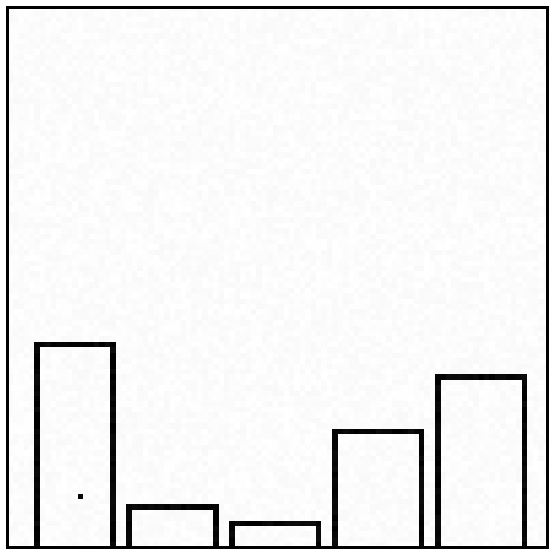
\includegraphics[width=.5in]{figure3_Bar_Chart.pdf}} & \makecell[tl]{Type 1: \emph{Bar Chart}\\~~~Perceptual Task: \emph{Position}\\~ \\~ \\} &~& \makecell[tr]{~\\ $878,520$}\\
%
%
%	\midrule
%	\raisebox{-.85\height}{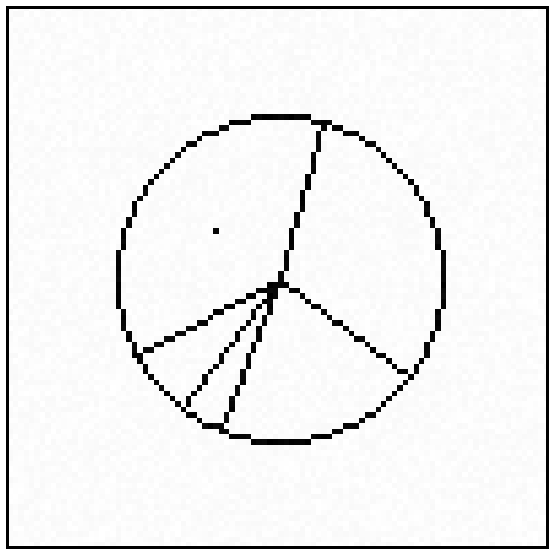
\includegraphics[width=.5in]{figure3_Pie_Chart.pdf}} & \makecell[tl]{Type 2: \emph{Pie Chart}\\~~~Perceptual Task: \emph{Angle}\\~ \\~ \\} &~& \makecell[tr]{~\\ $878,520$}\\
%
%
%	\bottomrule
%\end{tabular}
%}
%\label{tab:pos_angle_parameters}
%\end{table}

\subsection{Hypotheses}

\begin{hypolist}
	\item \textbf{H2.1} \textbf{Computed perceptual accuracy will be higher for bar charts than pie charts.} Cleveland and McGill report that position judgements are almost twice as accurate (MLAE) as angle judgements in humans. Following our ranking of elementary perceptual tasks (Table~\ref{tab:ranking}), we see that our networks also judge position encodings more accurately than angles, and so our networks will be able to more easily judge bar charts than pie charts.
	\item \textbf{H2.2} \textbf{Convolutional neural networks will learn to regress bar chart ratios faster than pie chart ratios in training.} This follows directly from H2.1.
\end{hypolist}

\subsection{Results}

\begin{figure}[t]
	\centering
	  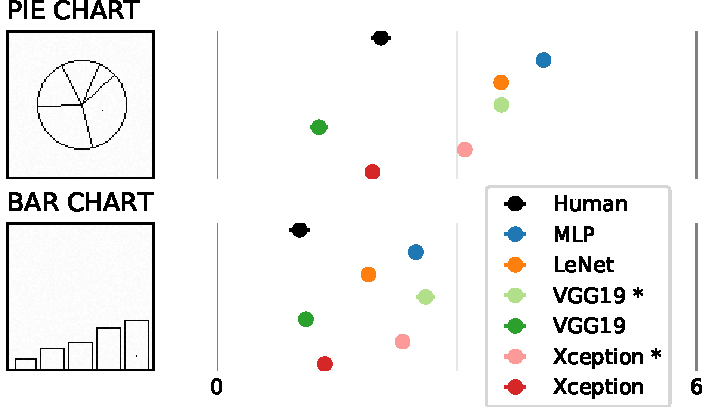
\includegraphics[width=\linewidth]{figure3_mlae_better_all.pdf}
  \caption{\textbf{Computational results of the position-angle experiment.} \textit{Left:} Our encodings of one data point as a pie chart and a bar chart. \textit{Right:} MLAE and 95\% confidence intervals for different networks. VGG19 * and Xception * are using ImageNet weights while all other networks were trained on the stimuli. We train all networks 12 times (4 times for VGG19 and Xception due to significantly longer training times). VGG19 * and Xception * use ImageNet weights. Our results align with Cleveland and McGill's human results, shown in black~\cite{cleveland_mcgill}.}
	\label{fig:figure3_mlae}
\end{figure}

% We evaluate over 56 runs for each condition \textit{visual encoding} (12 runs per network, but only 4 for VGG19 and Xception due to higher training times),

\noindent{\textbf{Perceptual Accuracy.}} Our networks are able to regress the task ratios for bar charts and pie charts (Fig.~\ref{fig:figure3_mlae}).  Cross-validation yields an average $MLAE=2.176$ ($SD=0.456$) for bar charts, and an average $MLAE=3.296$ ($SD=0.77$) for pie charts. This difference is statistically significant ($F_{1,110}=86.061, p<0.01$), and so we \textbf{accept H2.1}. 

Post hoc comparisons show that this holds for most networks: 
MLP for pie charts $4.09$ ($SD=0.027$) and for bar charts $2.494$ ($0.068$) is significant ($t_{22}=72.300,p<0.01$);
LeNet for pie charts $ 3.556 $ ($SD= 0.022 $) and for bar charts $ 1.902 $ ($SD= 0.08 $) is significant $t_{22}=66.111, p<0.01$;
VGG19 * with ImageNet weights for pie charts $ 3.561 $ ($SD= 0.047 $) and for bar charts $ 2.601 $ ($SD= 0.113 $) is significant $t_{22}=25.919,p<0.01$;
Xception * with ImageNet weights for pie charts  $ 3.094 $ ($SD= 0.046 $) and for bar charts $ 2.315 $ ($SD= 0.032 $) is significant $t_{22}=46.329,p<0.01$;
Xception from scratch for pie charts $ 1.939 $ ($SD= 0.1 $) and for bar charts $ 1.375 $ ($SD= 0.062 $) is significant $t_{22}=8.276,p<0.01$; but
the difference for VGG19 from scratch (pie charts $ 1.297 $ ($SD= 0.129 $), bar charts $ 1.153 $ ($SD= 0.09 $)) was not significant with $p<0.05$. 
This outcome is in line with the elementary perceptual task results (Table~\ref{tab:ranking}), where VGG19 was the most successful network, where networks trained from scratch were more performant, and where angle was more difficult to learn than position.
\\~\\
\noindent{\textbf{Training Efficiency.} We measure the MSE loss for all networks on previously-unseen validation data during training. We count a network as converged when this validation loss does not decrease after 10 sequential epochs. Figure~\ref{fig:figure3_val_loss} shows this MSE validation loss during the first twenty epochs for each condition, plotted across all cross-validation splits with overdrawn lines. The pie chart loss decreases more slowly, with the average loss over epochs being $0.052$ ($SD=0.015$) for pie charts and $0.037$ ($SD=0.018$) for bar charts. This difference is statistically significant ($F_{1,2238}=20.656, p<0.01$). Thus, we \textbf{accept H2.2}.
\\~\\
To all our networks, the bar chart is a superior visual encoding than a pie chart, in terms of accuracy and efficiency. Cleveland and McGill observe the same effect for accuracy during their human experiments.

% and conclude that the perceptual task of estimating position is easier for humans than the estimation of angles -> JT: Unless you have a direct quote, we're not putting words in their mouths. I couldn't find one in my brief look, but you might have one. If we do, then put a page number reference.

\begin{figure}[t]
	  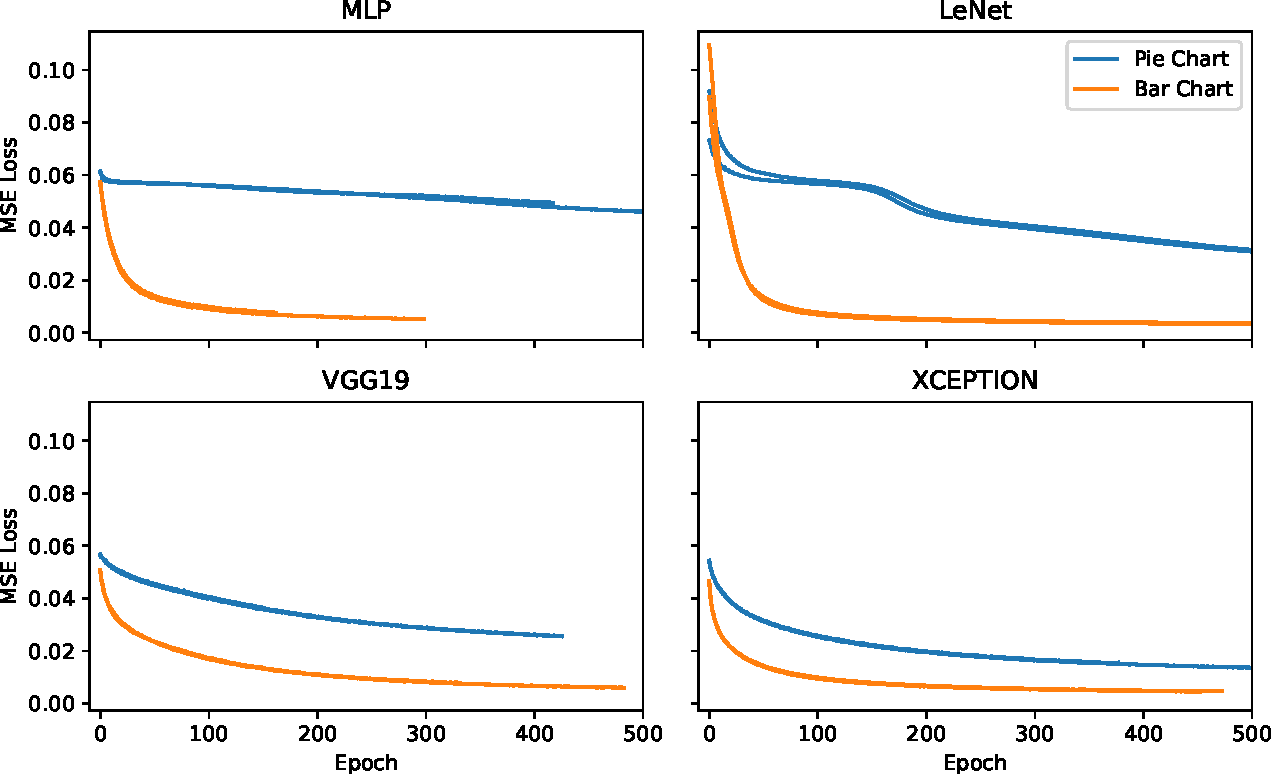
\includegraphics[width=\linewidth]{figure3_val_loss.pdf}
  \caption{\textbf{Training efficiency of the position-angle experiment.} Mean Squared Error (MSE) loss after each epoch during training, computed on previously-unseen validation data. We train all networks 12 times (4 times for VGG19 and Xception due to significantly longer training times). VGG19 * and Xception * use ImageNet weights. All networks converge faster when learning bar charts.}
	\label{fig:figure3_val_loss}
\end{figure}



\section{Position-Length Experiment}

This is the one where we estimate two selected bars compared to the longest one - very similar to the previous one but, not yet done. We basically test divided versus grouped barchart and we estimate one relation between two marked quanitities: what percent the smaller is of the larger.

There are five types: type 1-3 this is a position judgement along a common scale. (btw all classifiers seem to do that extremely well in the elementary tasks so we assume this will work well here too). Types 4-5 are length judgements and we know that the classifiers struggle with that quite a bit.

The setup from Cleveland McGill is first a classification task: which one is smaller? and then a regression task: how much smaller. So we have to see how to encode this.


\subsection{Hypotheses}

We proposed two hypotheses entering the elementary perceptual task experiment:

\begin{itemize}
	\item \textbf{H3.1} \textbf{Grouped bar charts are better computational perceivable than divided bar charts.} A grouped bar chart involves judging a position while a divided bar chart most likely (if not the bottom is looked at) requires length judgements. Classifiers are better at judging position than at judging length so grouped bar charts are easier to grasp in terms of computational perception.
	\item \textbf{H3.2} \textbf{not yet} Any ideas?
\end{itemize}


\begin{figure*}[t]
	  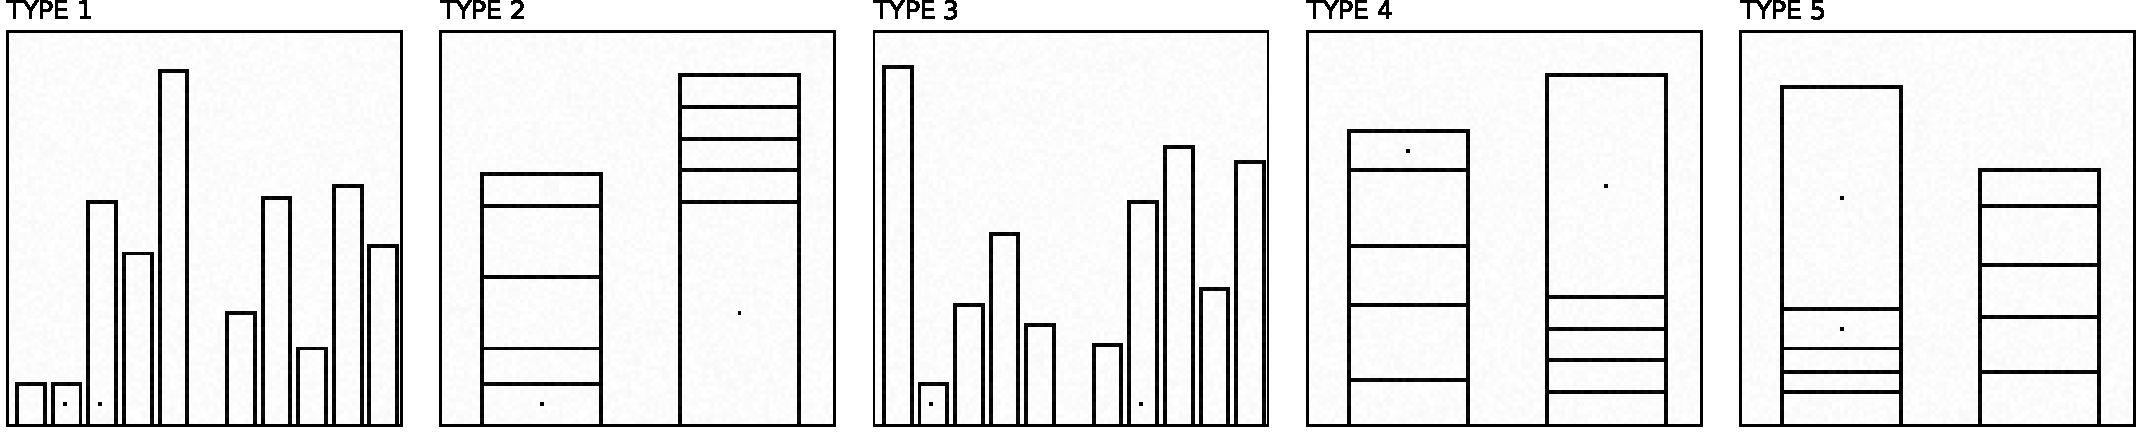
\includegraphics[width=\linewidth]{figure4_overview.pdf}
	  
  \caption{\textbf{Position-Length Experiment.} (Not yet) Rasterized versions of the graphs of Cleveland and McGill's position-length experiment. The perceptual task involves comparing. the two dot-marked quantities across five different visual encodings of either grouped or divided bar charts. We evaluate which type of bar chart performs better with our neural networks as a combined classification and regression problem. The first task is to select which of the marked quantities is smaller (classification) and the second task is to specify how much smaller it is (regression).}
	\label{fig:position_length_experiment}
\end{figure*}

\subsection{Discussion}

JT: Look at the relative difficulty of the tasks. In Cleveland and McGill, types 1-5 were post-ordered by their log error such that type 1 was easiest and type 5 was hardest. Is this still the case with our CNNs?

\subsection{Results}


\begin{figure}[t]
	  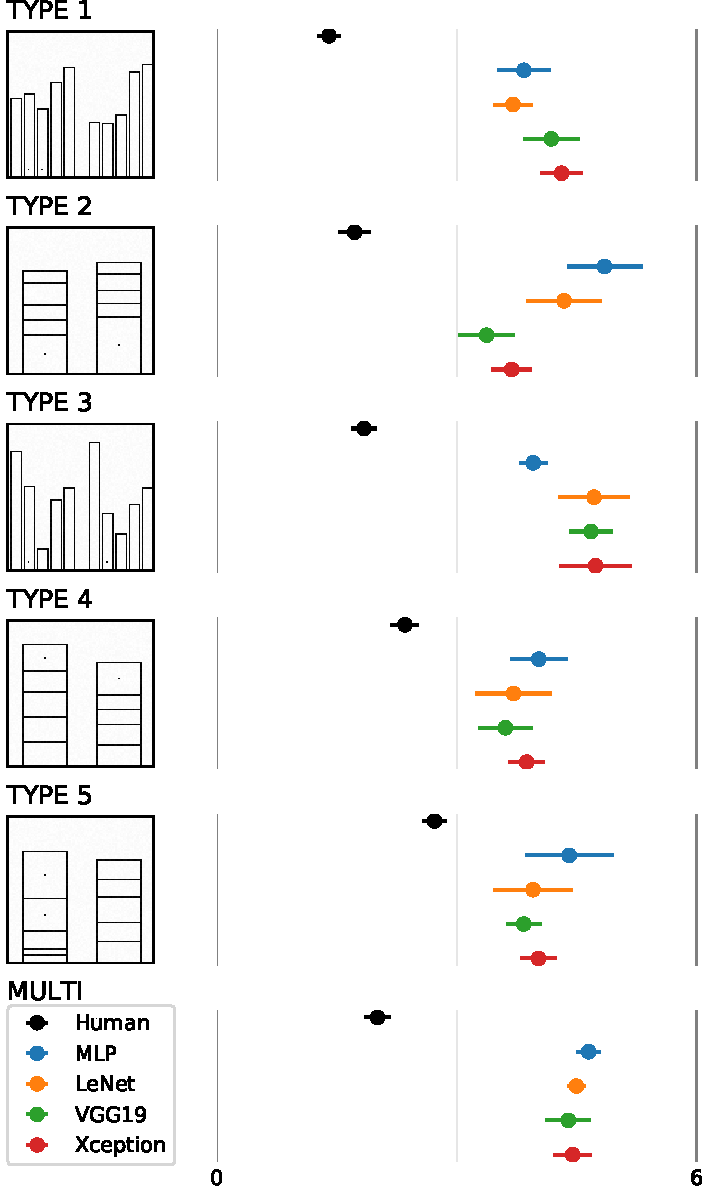
\includegraphics[width=\linewidth]{figure4_mlae_with_multi_and_humans.pdf}
  \caption{\textbf{Computational results of the Position-Length experiment.} Log absolute error means and 95\% confidence intervals for the \emph{position-length experiment} as described by Cleveland and McGill~\cite{cleveland_mcgill}. We test the performance of a Multi-layer Perceptron (MLP), the LeNet Convolutional Neural Network, as well as feature generation using the VGG19 and Xception networks trained on ImageNet.}
	\label{fig:figure4_mlae}
\end{figure}


\section{Bars and Framed Rectangles Experiment}

Visual cues can help converting graphical elements back to their real world variables. Cleveland and McGill introduced the bars and framed rectangles experiment which judges the elementary perceptual task of position along non-aligned scales~\cite{cleveland_mcgill}. 

\subsection{Hypotheses}

We proposed two hypotheses entering the elementary perceptual task experiment:

\begin{itemize}
	\item \textbf{H4.1} \textbf{Classifiers can leverage additional visual cues.} The original bar and framed rectangle experiment shows how visual cues aid humans in mapping graphical elements to quantitative variables. This should be the same for feed-forward neural networks since they are inspired by the visual system.
	\item \textbf{H4.2} \textbf{Weber's law can be transferred to computational perception.} Cleveland and McGill confirmed Weber's law based on the bar and framed rectangle experiment. For humans, the ability to perceive change within a distribution is proportional to the size of the initial distribution.
\end{itemize}

\begin{figure}[t]
	  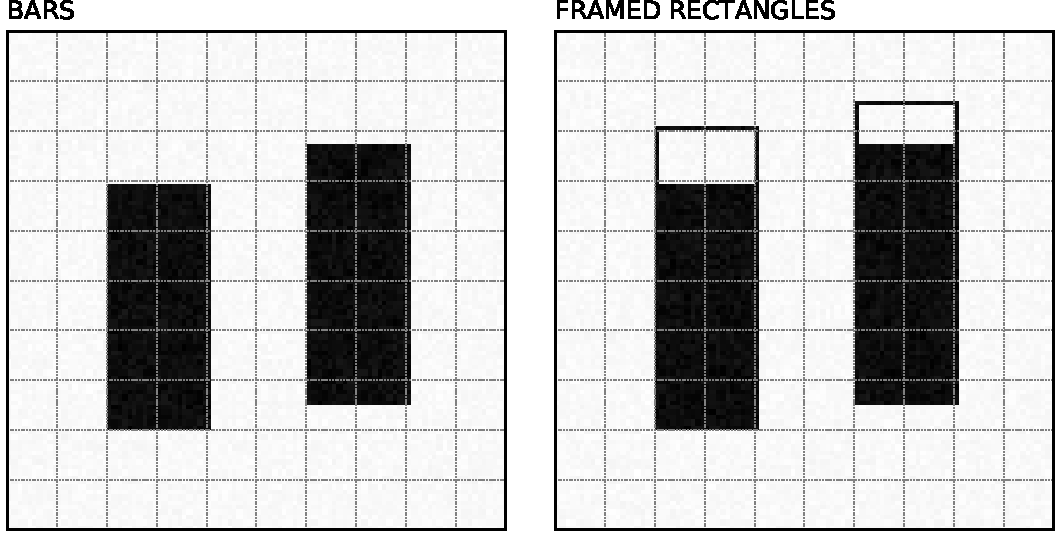
\includegraphics[width=\linewidth]{figure12_overview}
  \caption{\textbf{Bars and Framed Rectangles Experiment.} Cleveland and McGill introduce the bars and framed rectangles experiment which measures the perceptual task of judging position along non-aligned scales. For humans, it is easier to decide which of two bars represent a larger height if a scale is introduced by adding framed rectangles (right). In this case, the right bar is heigher as visible with less free space when adding the frame. We evaluate whether such a visual aid also helps machines to perceive visually encoded quantities.}
	\label{fig:bars_and_framed_rectangles_experiment}
\end{figure}

\subsection{Weber-Fechner's Law}

As identified by Cleveland and McGill, the bar and framed rectangle experiment is closely related to Weber's law. This psychophysics law states that perceivable difference within a distribution is proportional to the initial size of the distribution. Weber's law goes hand-in-hand with Fechner's law. We conduct an additional experiment based on the original illustrations of the Weber-Fechner law to investigate whether this law can be applied to computational perception of our classifiers (Fig.~\ref{fig:webers_law}).

\begin{figure}[t]
	  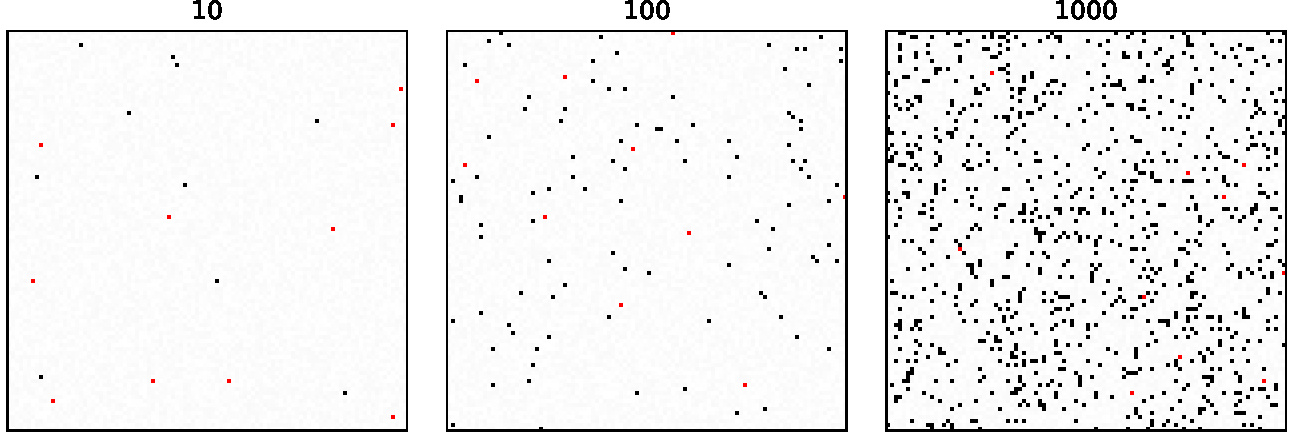
\includegraphics[width=\linewidth]{weber_overview}
  \caption{\textbf{Weber-Fechner Law.} The Weber-Fechner law states that the perceivable differences within a distribution is proportional to the initial size of the distribution. The lower square contains 10 more dots than the upper one on both sides. However, the difference is easily perceivable on the left while the squares on the right almost look the same. We generate rasterized visualizations similar to this setup and evaluate our classifiers.}
	\label{fig:webers_law}
\end{figure}

\subsection{Results}

First run indicates that framed rectangles perform better but we dont really know it yet.

\begin{figure*}[t]
	  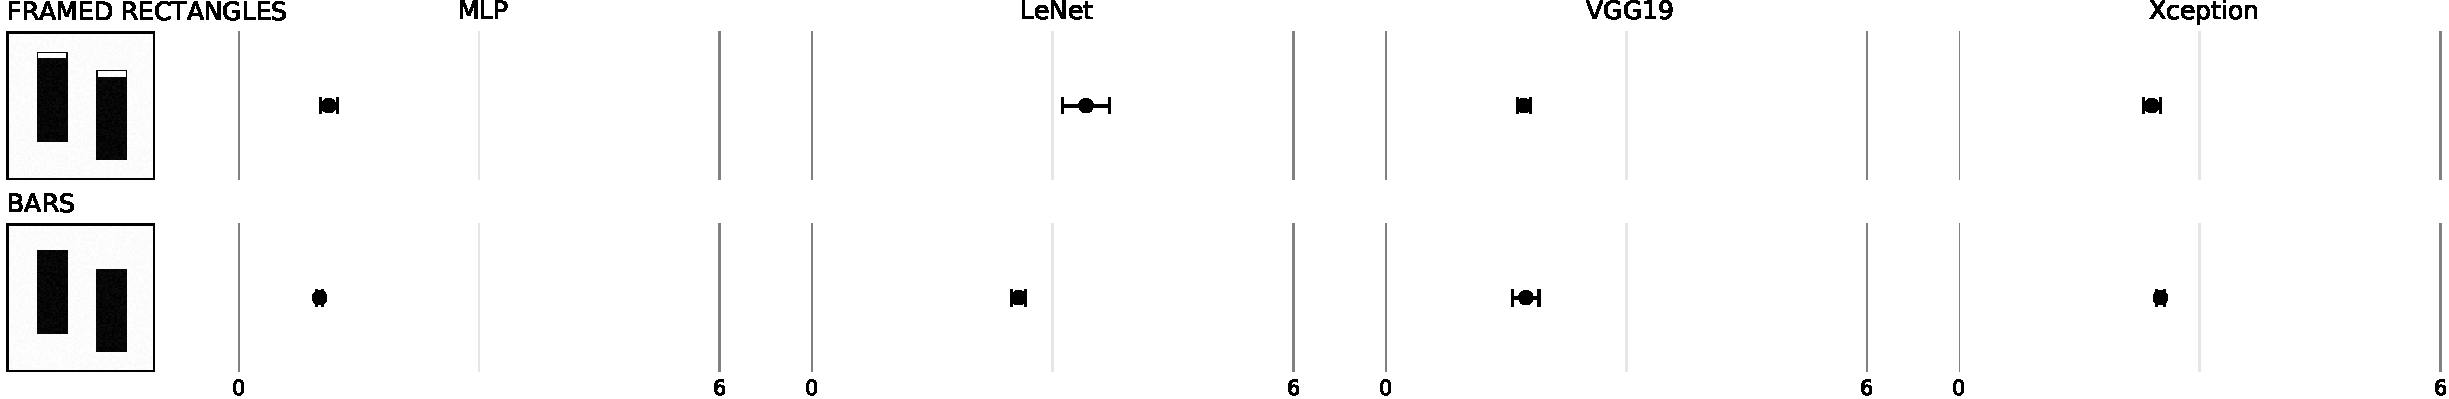
\includegraphics[width=\linewidth]{figure12_mlae.pdf}
  \caption{\textbf{Computational results of the Bars-and-Framed-Rectangles experiment.} Log absolute error means and 95\% confidence intervals for the \emph{bars-and-framed-rectangles experiment} as described by Cleveland and McGill~\cite{cleveland_mcgill}. We test the performance of a Multi-layer Perceptron (MLP), the LeNet Convolutional Neural Network, as well as feature generation using the VGG19 and Xception networks trained on ImageNet.}
	\label{fig:figure12_mlae}
\end{figure*}



\section{Results and Discussion}

\subsection{Elementary Perceptual Tasks}

some are good and some are bad.. why?

\begin{figure*}[h]
	  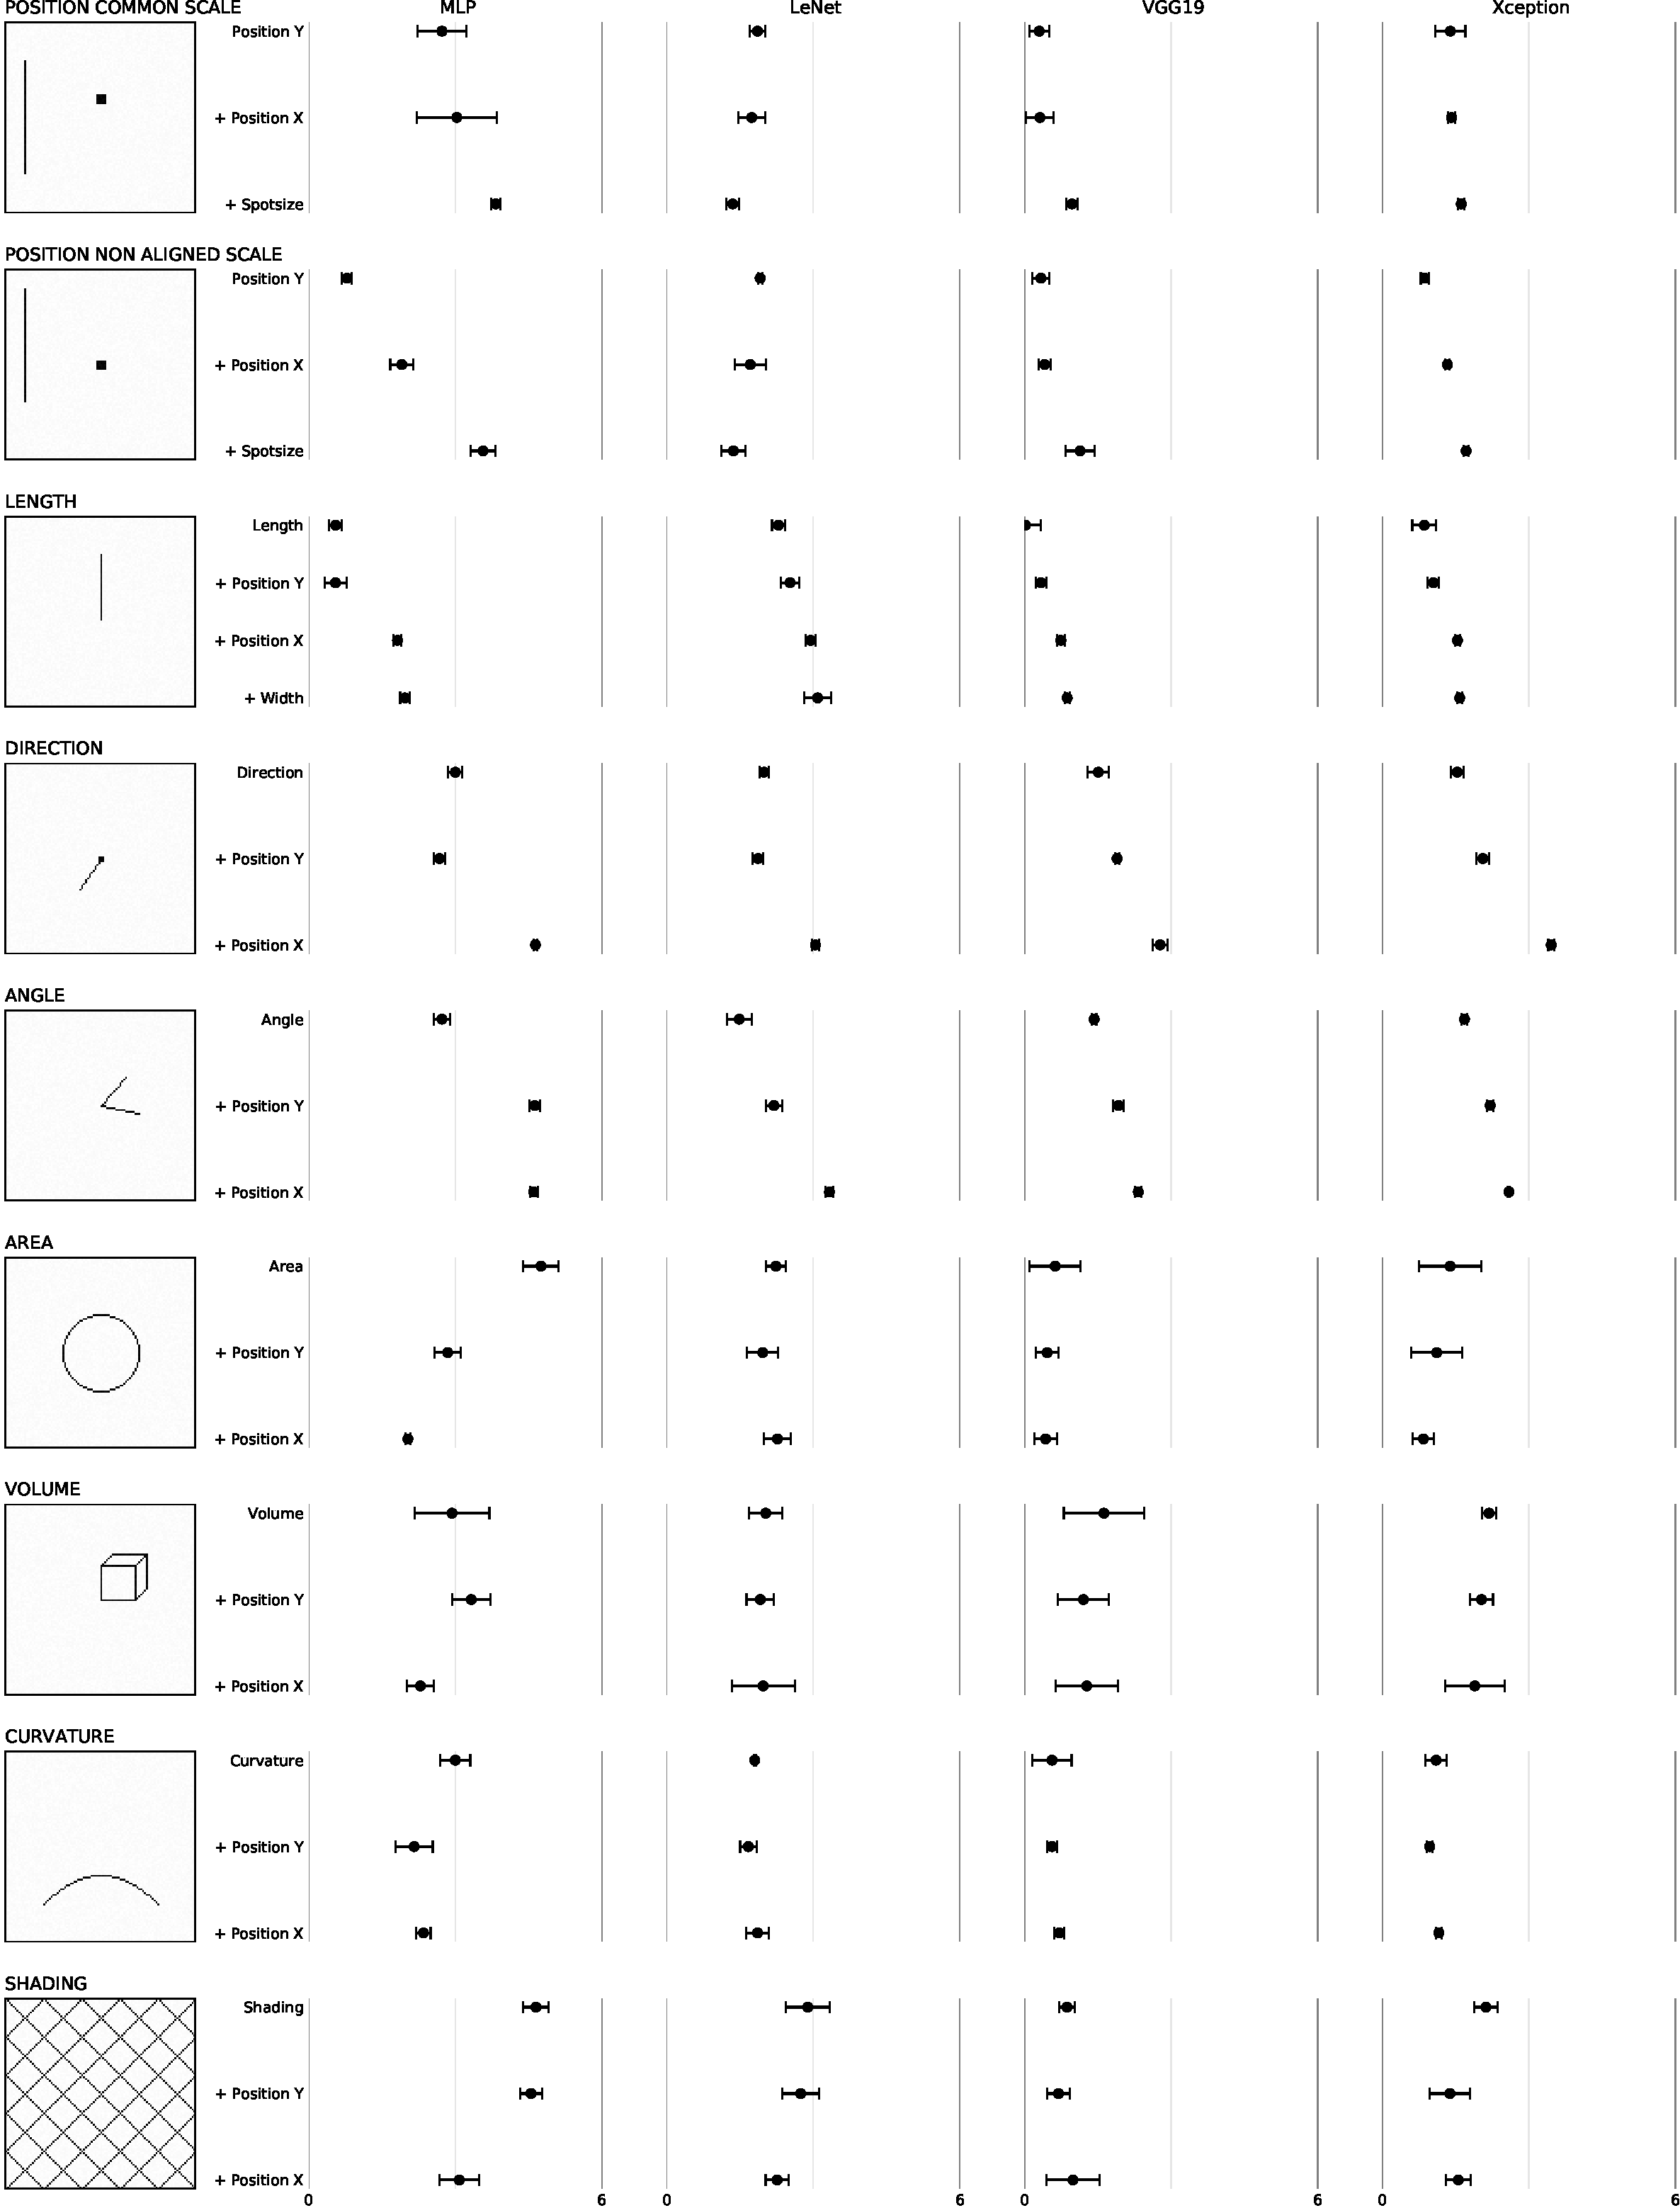
\includegraphics[width=\linewidth]{figure1_latest.pdf}
  \caption{\textbf{Computational results of Elementary Perceptual Tasks experiment.} Log absolute error means and 95\% confidence intervals for computed perception of different classifiers on the \emph{elementary perceptual tasks} introduced by Cleveland and McGill 1984~\cite{cleveland_mcgill}. We test the performance of a Multi-layer Perceptron (MLP), the LeNet Convolutional Neural Network, as well as feature generation using the VGG19 and Xception networks trained on ImageNet.}
	\label{fig:figure1_results}
\end{figure*}

\textbf{Computational Perception Ranking.}

Cleveland McGills Ranking - can we observe something similar?

\begin{enumerate}
	\item Position along a common scale e.g. scatter plot
	\item Position on identical but nonaligned scales e.g. multiple scatter plots
	\item Length e.g. bar chart
	\item Angle \& Slope (tie) e.g. pie chart
	\item Area e.g. bubbles
	\item Volume, density, and color saturation (tie) e.g. heatmap
	\item Color hue e.g. newsmap
\end{enumerate}

\noindent{\textbf{Cross-classifier variability.}}

Can a neural network generalize on simple perceptual tasks?

\begin{figure}[t]
	  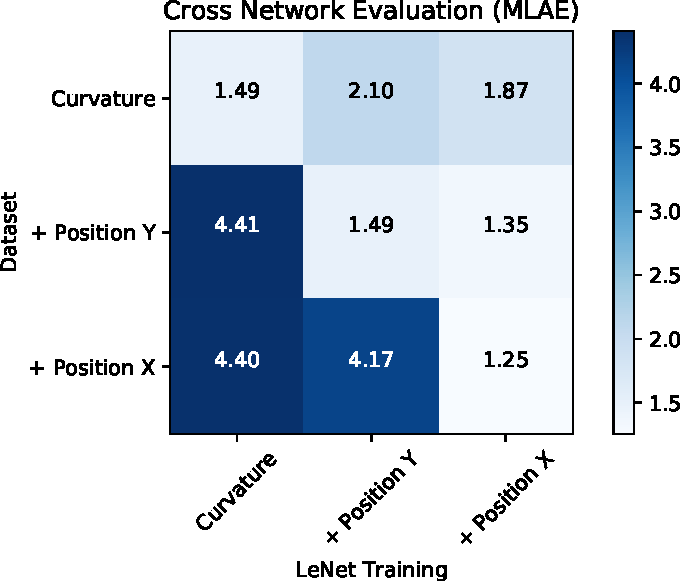
\includegraphics[width=\linewidth]{crossnetwork.pdf}
  \caption{\textbf{Cross-classifier variability for the perceptual task of measuring curvature.} We use predictions of LeNet classifiers trained on different parametrizations of the \emph{curvature} elementary perceptual task and measure the mean logistic absolute error (MLAE). The lower score, the better. Classifiers trained on curves with variable position can generalize even if the axis of translation varies. However, classifiers trained on fixed positions of curves are not able to measure translated curves.}
	\label{fig:cross_network}
\end{figure}


\subsection{Position-Angle Experiment}

Bar charts are more accurate (Fig.~\ref{fig:figure3_mlae}) and networks converge faster (Fig.~\ref{fig:figure3_val_loss}). This is great.

\begin{figure}[t]
	  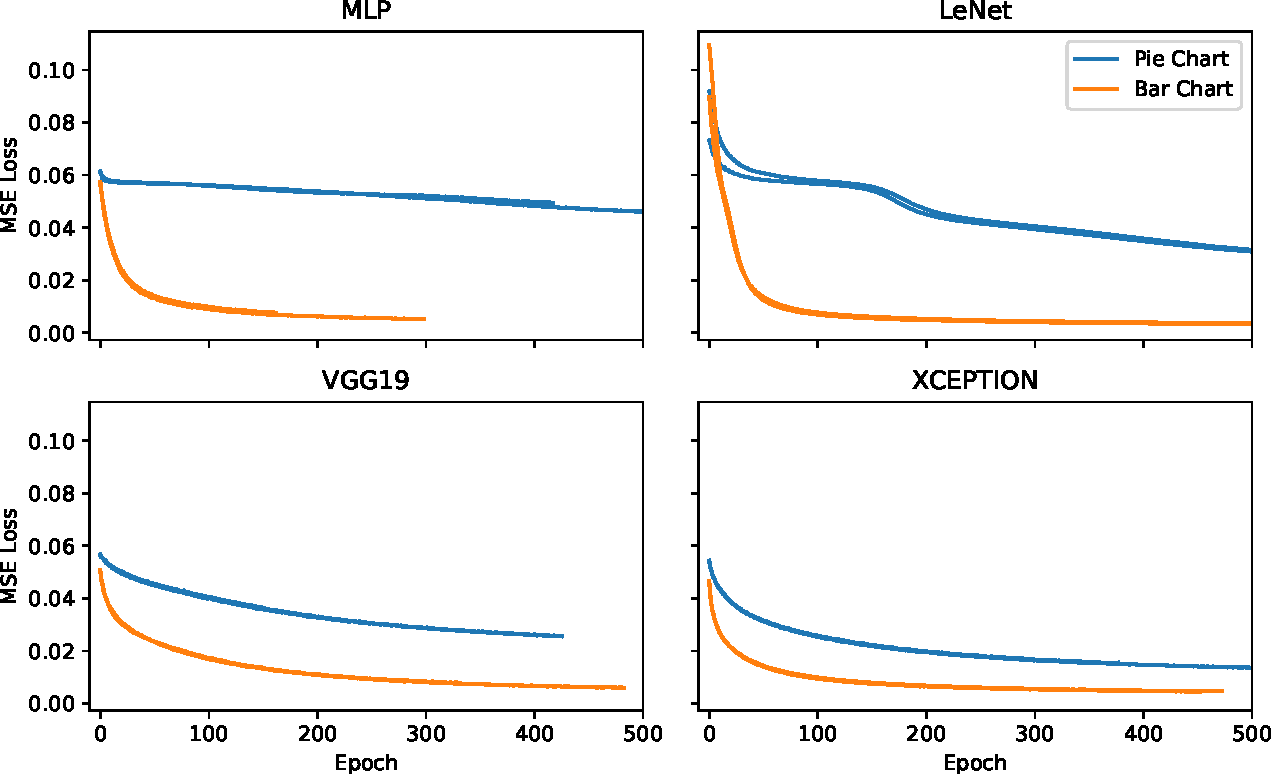
\includegraphics[width=\linewidth]{figure3_val_loss.pdf}
  \caption{\textbf{Classifier Efficiency of the Position-Angle experiment.} Mean Square Error (MSE) loss for the \emph{position-angle experiment} as described by Cleveland and McGill~\cite{cleveland_mcgill} which compares the visualization of pie charts and bar charts. We report the MSE measure for both encodings of four different classifier on previously unseen validation data.}
	\label{fig:figure3_val_loss}
\end{figure}

\begin{figure*}[t]
	  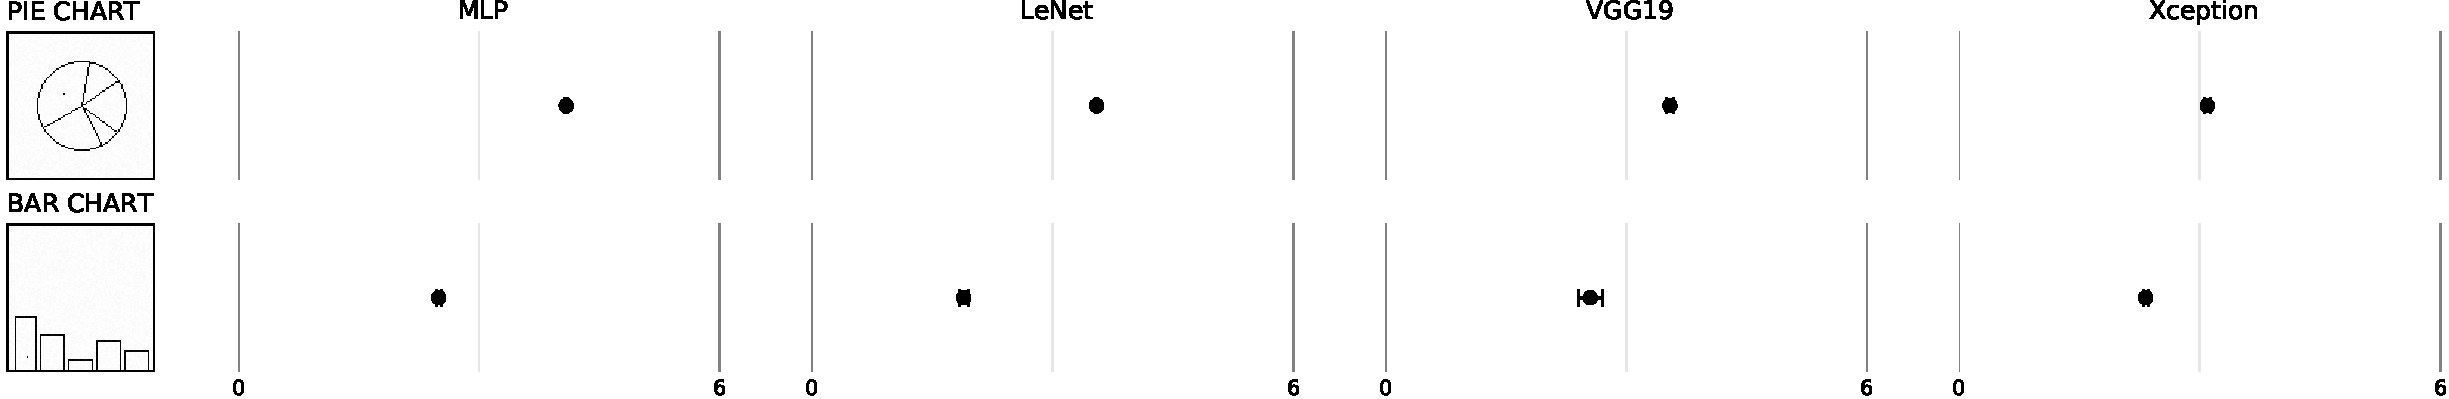
\includegraphics[width=\linewidth]{figure3_mlae.pdf}
  \caption{\textbf{Computational results of the Position-Angle experiment.} Log absolute error means and 95\% confidence intervals for the \emph{position-angle experiment} as described by Cleveland and McGill~\cite{cleveland_mcgill}. We test the performance of a Multi-layer Perceptron (MLP), the LeNet Convolutional Neural Network, as well as feature generation using the VGG19 and Xception networks trained on ImageNet.}
	\label{fig:figure3_mlae}
\end{figure*}

\subsection{Position-Length Experiment}

\begin{figure*}[t]
	  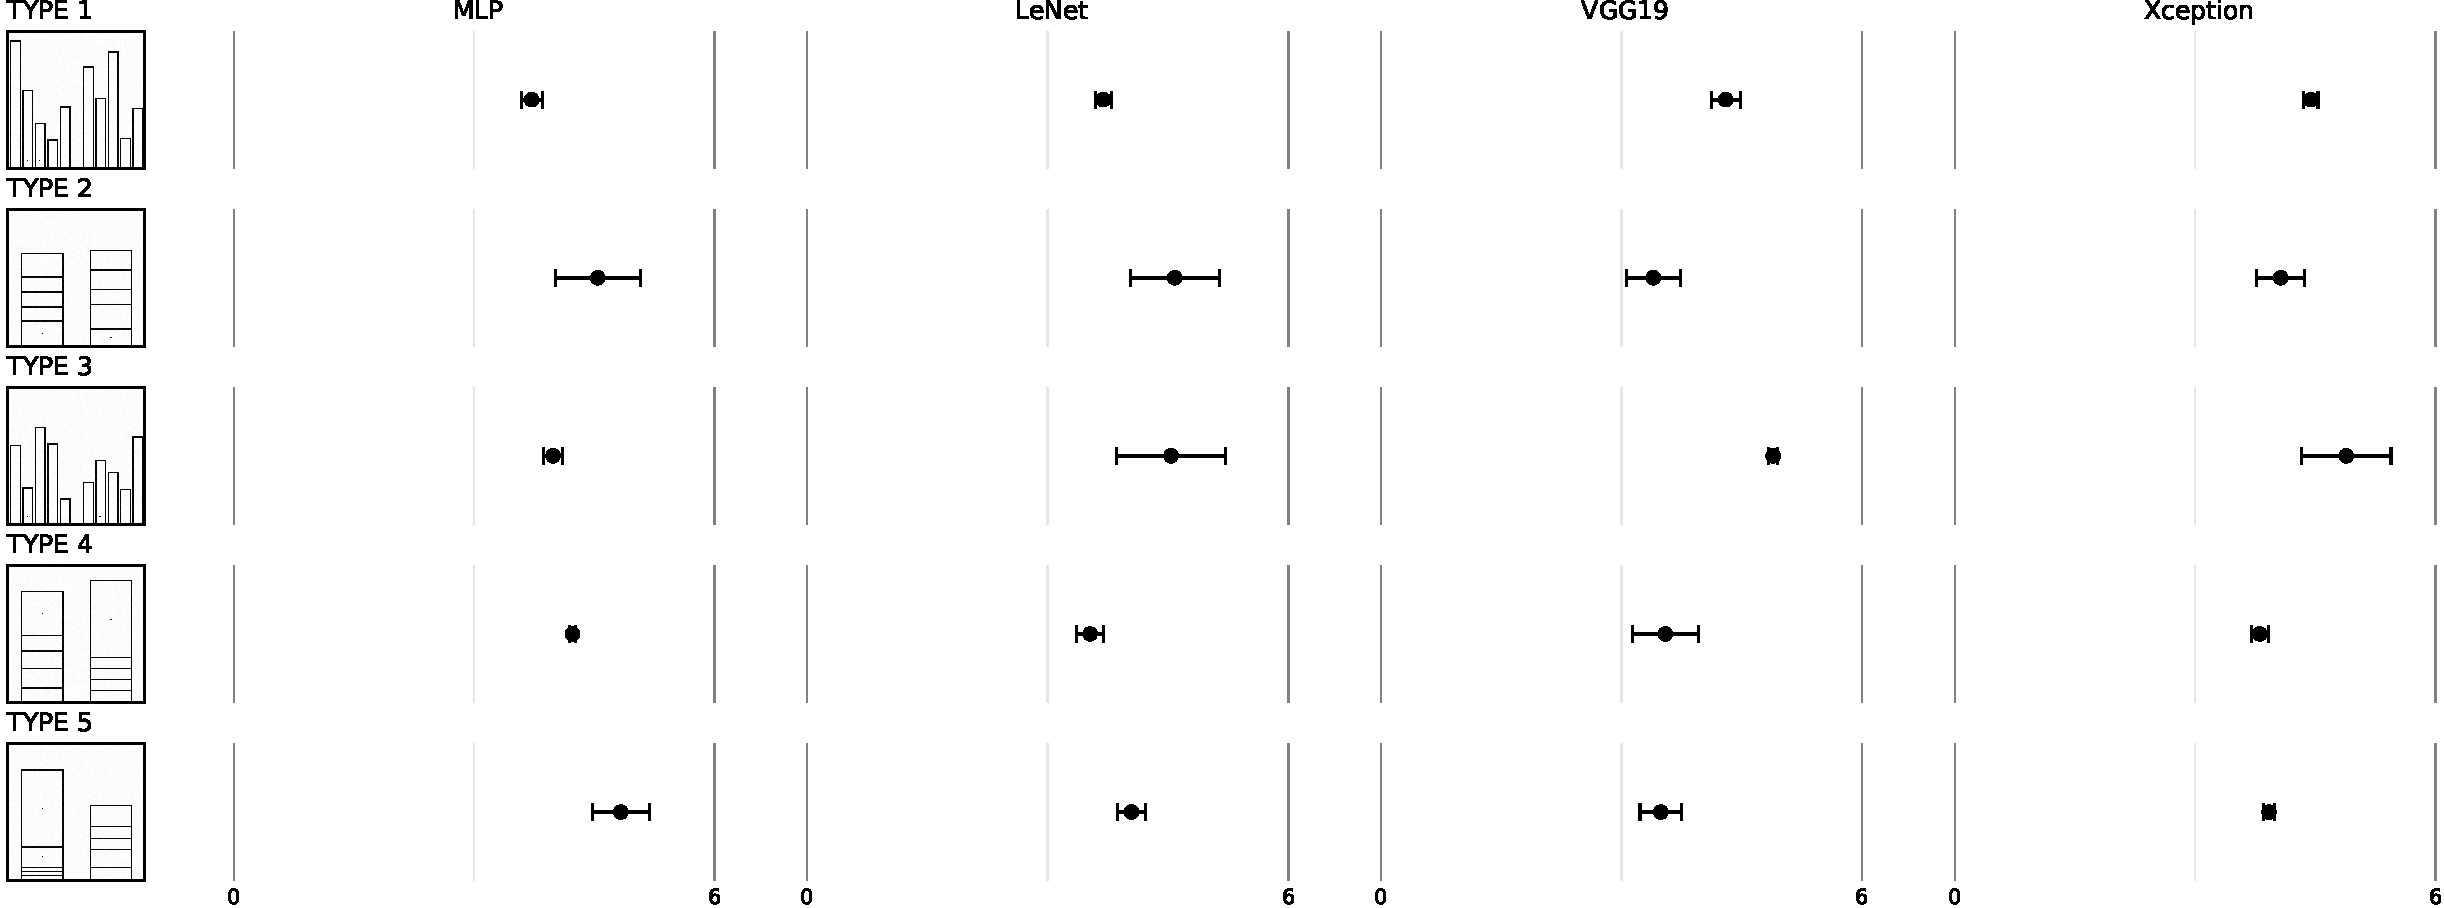
\includegraphics[width=\linewidth]{figure4_mlae.pdf}
  \caption{\textbf{Computational results of the Position-Length experiment.} Log absolute error means and 95\% confidence intervals for the \emph{position-length experiment} as described by Cleveland and McGill~\cite{cleveland_mcgill}. We test the performance of a Multi-layer Perceptron (MLP), the LeNet Convolutional Neural Network, as well as feature generation using the VGG19 and Xception networks trained on ImageNet.}
	\label{fig:figure4_mlae}
\end{figure*}

\subsection{Bars and Framed Rectangles Experiment}

First run indicates that framed rectangles perform better but we dont really know it yet.

\begin{figure*}[t]
	  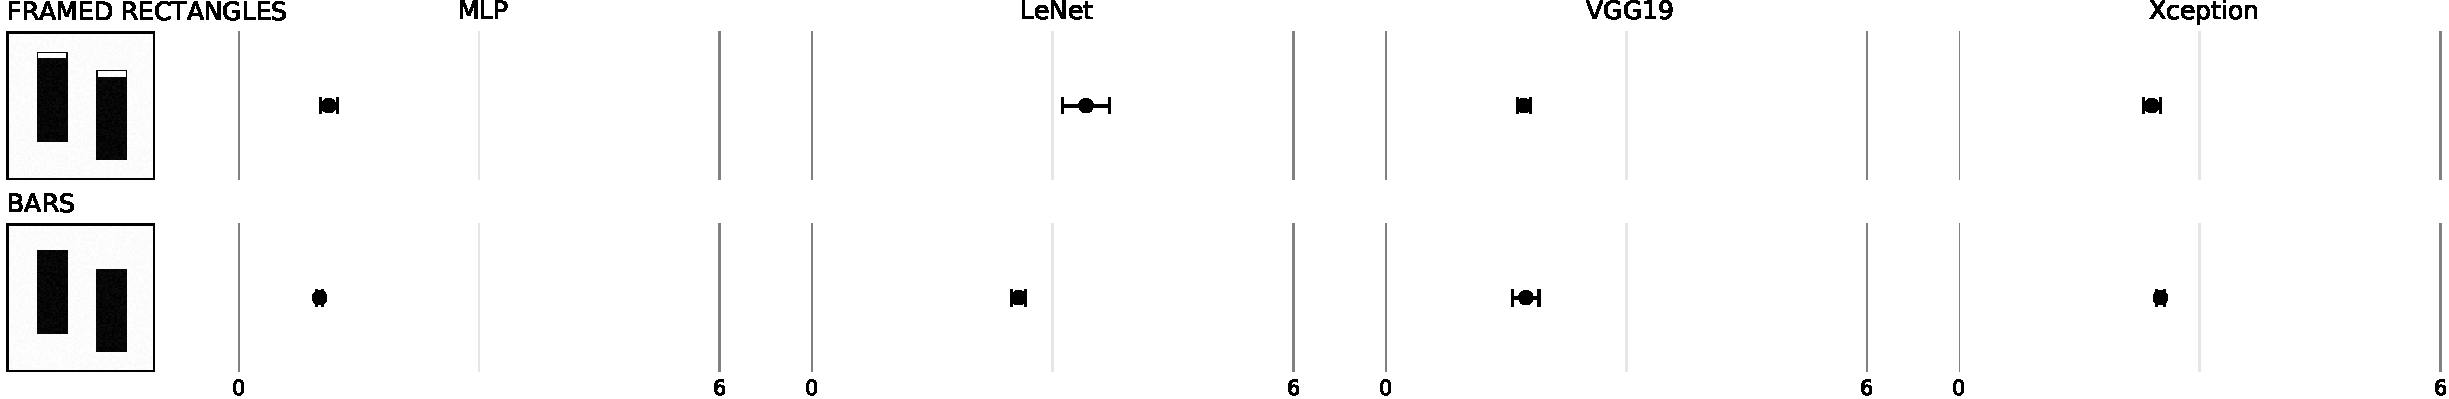
\includegraphics[width=\linewidth]{figure12_mlae.pdf}
  \caption{\textbf{Computational results of the Bars-and-Framed-Rectangles experiment.} Log absolute error means and 95\% confidence intervals for the \emph{bars-and-framed-rectangles experiment} as described by Cleveland and McGill~\cite{cleveland_mcgill}. We test the performance of a Multi-layer Perceptron (MLP), the LeNet Convolutional Neural Network, as well as feature generation using the VGG19 and Xception networks trained on ImageNet.}
	\label{fig:figure12_mlae}
\end{figure*}

\begin{figure}[t]
	  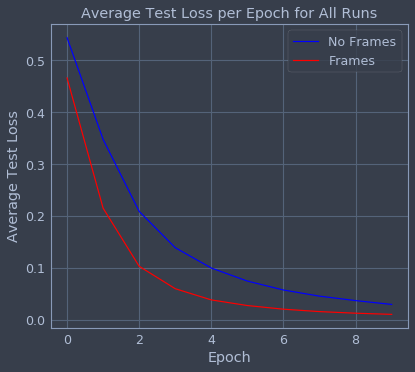
\includegraphics[width=\linewidth]{figure12_val_loss.png}
  \caption{\textbf{Classifier Efficiency of the Bars and Framed Rectangles experiment.} Categorical Cross-Entropy loss for the \emph{bars and framed rectangles experiment} as described by Cleveland and McGill~\cite{cleveland_mcgill}. The frame around the bars adds an additional visual cue enables faster network convergence. This is not yet reproducible!}
	\label{fig:figure12_val_loss}
\end{figure}


\section{Conclusions}

Future work: allow insights for infovis for machines



%% if specified like this the section will be committed in review mode
%\acknowledgments{
%The authors wish to thank A, B, and C. This work was supported in part by
%a grant from XYZ (\# 12345-67890).}

%\bibliographystyle{abbrv}
\bibliographystyle{abbrv-doi}
%\bibliographystyle{abbrv-doi-narrow}
%\bibliographystyle{abbrv-doi-hyperref}
%\bibliographystyle{abbrv-doi-hyperref-narrow}

\bibliography{paper.bib}
\end{document}

